\documentclass[fontsize=10pt,paper=A5,twoside,BCOR=1mm,DIV=21,headinclude]{scrarticle}
%\usepackage{calligra}
\usepackage{breviarium}
\usepackage[german]{babel}
%\usepackage[autocompile]{gregoriotex}
%\usepackage{mathtools}
%\usepackage{pdfpages}
\newcommand{\DHSME}{\V Der Herr sei mit euch. \R Und mit deinem Geiste.}
\newcommand{\DHL}{\DHSME

\hfill\red{L}asset uns beten.\hfill\null}
\newcommand{\position}[1]{{
\centering \rubric{– \textit{#1} –}

}}
\renewcommand{\hora}[1]{
	\addcontentsline{toc}{section}{#1}
	\chead{#1}
	\vspace{.5em}
	{\centering\small{\uppercase{#1}}

		\vspace{.5em}
	}
}
\newcommand{\tempvar}{}
\renewcommand{\die}[4]{
	\addcontentsline{toc}{subsection}{#2 #4}
	{\centering 
		\vspace{-0.3em}

		\noindent\rule{0.45 \textwidth}{.5pt}

		\vspace{0.2em}

		#1

		{\large{#2}}

		\ifthenelse{\equal{#3}{}}{\vspace{-1.1em}}{} {\textcolor{red}{#3}}

	}
	\chead{\trim{#1}{#2}}
}
\renewcommand{\dieii}[4]{
	\addcontentsline{toc}{subsection}{#2 #4}


	\vspace{1em}

	{\centering 

		#1

		{\large{#2}}

		\ifthenelse{\equal{#3}{}}{\vspace{-1.1em}}{} {\textcolor{red}{#3}}

	}
	\chead{\trim{#1}{#2}}
}


\addto\captionsgerman{\renewcommand{\contentsname}{Inhalt}}
\begin{document}
\thispagestyle{empty}
{\centering\Large
	\null

	\vspace{2em}

	Matthäus Freitag

	\vspace{.5em}

	Rafael Suppmann

	%\vspace{2em}
	\vfill

	\LARGE Komplet

	\vspace{1em}

	\Large Nach dem Paderborner Brevier von 1513
	
	\vfill
}
\pagebreak 
\thispagestyle{empty}
\null
\pagebreak
\thispagestyle{empty}
{\centering\LARGE
	\null

	\vspace{2em}

	Matthäus Freitag

	\vspace{.5em}

	Rafael Suppmann

	%\vspace{2em}
	\vfill

	\Huge Komplet

	\vspace{1em}

	\LARGE Nach dem Paderborner Brevier von 1513
	
	\vfill

	\vspace{2em}

	\Large Paderborn 2024

	\vspace{2em}
\pagebreak 
\thispagestyle{empty}
\null

	\vfill

	\large Veröffentlichungen der\\Erzbischöflichen Akademischen Bibliothek\\Paderborn

	\vspace{.5em}

	Herausgegeben vom Direktor der Bibliothek\\
	Prof. Dr. Hans-Walter Stork

	\vspace{1.5em}

	Heft ???

	\vspace{3em}

}
\pagebreak
\thispagestyle{empty}
\null 

\vspace*{-1.4cm}

\tableofcontents

%\vfill

\null 

\pagebreak
\thispagestyle{empty}
\null

\vspace*{-1cm}
\mensii{Ad Completorium}

%\begin{center}
%	\begin{tikzpicture}[remember picture]
%		\node at (0,0) {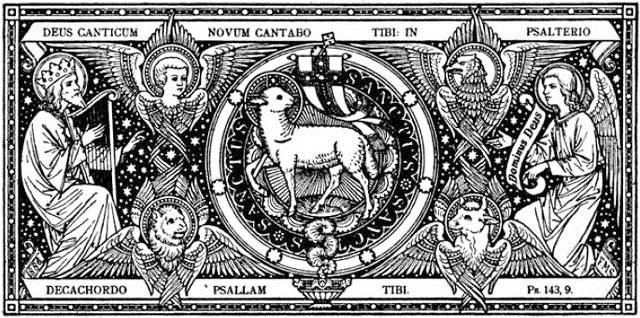
\includegraphics[width=0.90\linewidth]{Lithographie-Lamm-Evangelisten.jpg}};
%	\end{tikzpicture}
%\end{center}
%\null

%\vspace{-1.2em}

\hora{Eröffnung}

\vspace{.3em}

\begin{paracol}{2}
	\pcb
	\y{C}{onverte} nos Deus salutáris noster.
	\R Et avérte iram tuam a nobis.

	\V Deus in adjutórium meum inténde.
	\R Dómine ad adjuvándum me festína.
	\red{G}lória Patri et Fílio, * et Spirítui Sancto.
	\red{S}icut erat in princípio, et nunc, et semper, * et in s\'æcula sæculórum. Amen.
	\red{A}llelúja.
	\red{vel a Septuagesima usque ad Pascham L}aus tibi, Dómine, \f Rex ætérnæ glóriæ.
\switchcolumn
	\y{B}{ekehre} uns, Gott, unser Heil.
	\R Und wende Deinen Zorn von uns ab.

	\V O Gott, komm mir zu Hilfe.
	\R Herr, eile, mir zu helfen.
	\red{E}hre sei dem Vater und dem Sohn * und dem Heiligen Geist.
	\red{W}ie im Anfang, so auch jetzt und alle Zeit * und in Ewigkeit. Amen.
	\red{A}llelúja.
	\red{oder von Septuagesima bis Ostern: L}ob sei dir, Herr, König der ewigen Herrlichkeit.
\end{paracol}

\hora{Psalmodie}

\pars{Psalm 4}

\vspace{.3em}

\begin{paracol}{2} \pcb
\begin{psalmus}

\Y{C}{um} invocárem~exaudívit me Deus justítiæ meæ: * in tribulatióne dilatásti mihi.
	\switchcolumn
	\yb{D}{a} ich rief, erhörte mich der Gott meiner Gerechtigkeit; * in der Trübsal hast Du mir Raum gemacht.
\switchcolumn*
Miserére mei, * et exáudi oratiónem meam.
	\switchcolumn
	Erbarme Dich meiner * und erhöre mein Gebet.
\switchcolumn*
Fílii hóminum, úsquequo gravi corde? * ut quid dilígitis vanitátem, et quǽritis mendácium?

Et scitóte quóniam mirificávit Dóminus sanctum suum: * Dóminus exáudiet me cum clamávero ad eum.
	\switchcolumn
	Ihr Menschenkinder! wie lange ist noch schwer euer Herz? * Warum liebt ihr die Eitelkeit, und suchet die Lüge?

	Wisset doch, dass der Herr Wunder getan an Seinem Heiligen; * der Herr höret mich, wenn ich zu Ihm rufe.
\switchcolumn*
Irascímini, et nolíte peccáre: * quæ dícitis in córdibus vestris, in cubílibus vestris compungímini.
	\switchcolumn
	Zürnet ihr, so sündiget nicht; * was ihr sprechet in eurem Herzen, das bereuet auf euern Lagern.
\switchcolumn*
Sacrificáte sacrifícium justítiæ, et speráte in Dómino. * Multi dicunt: Quis osténdit nobis bona?

Signátum est super nos lumen vultus tui, Dómine: * dedísti lætítiam in corde meo.
	\switchcolumn
	Opfert ein Opfer der Gerechtigkeit, und hoffet auf den Herrn! * Viele sagen: Wer wird uns Gutes sehen lassen?

	Das Licht Deines Angesichtes ist gezeichnet über uns, o Herr; * Du hast Freude in mein Herz gegeben!
\switchcolumn*
A fructu fruménti, vini, et ólei sui * multiplicáti sunt.

In pace in idípsum * dórmiam, et requiéscam;

Quóniam tu, Dómine, singuláriter in spe * constituísti me.
	
Glória Patri, et Fílio, * et Spirítui Sancto.
	\switchcolumn
	Von der Frucht des Getreides, des Weines, und ihres Öles * sind sie reich geworden.

	In Frieden zugleich * werde ich schlafen und ruhen.

	Denn Du, Herr, hast mich in der Hoffnung * beispiellos festgestellt.

	Ehre sei dem Vater und dem Sohn * und dem Heiligen Geist.
\switchcolumn*
Sicut erat in princípio, et nunc et semper, * et in s\'æcula sæculórum. Amen.
	\switchcolumn
	Wie im Anfang, so auch jetzt und alle Zeit * und in Ewigkeit. Amen.
\end{psalmus}
\end{paracol}

\pars{Psalm 30, 1-6}

\vspace{.3em}

\begin{paracol}{2} \pcb
\begin{psalmus}
\y{I}{n} te, Dómine, sperávi, non confúndar in ætérnum: * in justítia tua líbera me.

	\switchcolumn 
	\y{A}{uf} Dich, o Herr, habe ich gehofft; möge ich niemals zuschanden werden; * in Deiner Gerechtigkeit befreie mich.
\switchcolumn*
Inclína ad me aurem tuam, * accélera ut éruas me.

Esto mihi in Deum protectórem, et in domum refúgii: * ut salvum me fácias.
	\switchcolumn 
	Neige Dein Ohr zu mir, * eile, mich zu erretten!

	Sei mir ein schirmender Gott und eine Stätte der Zuflucht, * auf dass Du mir Heil verschaffst!
\switchcolumn*
Quóniam fortitúdo mea, et refúgium meum es tu: * et propter nomen tuum dedúces me, et enútries me.

Edúces me de láqueo hoc, quem abscondérunt mihi: * quóniam tu es protéctor meus.

In manus tuas comméndo spíritum meum: * redemísti me, Dómine, Deus veritátis.

%Odísti observántes vanitátes, * supervácue.

%Ego autem in Dómino sperávi: * exsultábo, et lætábor in misericórdia tua.
	\switchcolumn 
	Denn Du bist meine Stärke und meine Zuflucht, * und um Deines Namens willen mögest Du mich leiten und nähren.

	Du wirst mich aus der Schlinge ziehen, die man mir heimlich gelegt hat; * denn Du bist mein Beschirmer.

	In Deine Hände befehle ich meinen Geist: * Du hast mich erlöst, o Herr, Gott der Treue.

%	Verhaß sind Dir die Verehrer * nichtiger Götzen.

%	Ich aber schenke dem Herrn mein Vertrauen: * Freudig will ich frohlocken ob Deiner Huld.
%\switchcolumn*
%Quóniam respexísti humilitátem meam, * salvásti de necessitátibus ánimam meam.

%Nec conclusísti me in mánibus inimíci: * statuísti in loco spatióso pedes meos.
%	\switchcolumn
%	Daß Du mein Elend geschaut, * meiner Seele Nöte beachtet hast.

%	Daß Du mich nicht der Feindeshand überliefert, * sondern auf freien Ort meine Füße gestellt hast.
%\switchcolumn*
%Miserére mei, Dómine, quóniam tríbulor: * conturbátus est in ira óculus meus, ánima mea, et venter meus:

%Quóniam defécit in dolóre vita mea: * et anni mei in gemítibus.

%Infirmáta est in paupertáte virtus mea: * et ossa mea conturbáta sunt.

%Super omnes inimícos meos factus sum oppróbrium et vicínis meis valde: * et timor notis meis.

%Qui vidébant me, foras fugérunt a me: * oblivióni datus sum, tamquam mórtuus a corde.

%Factus sum tamquam vas pérditum: * quóniam audívi vituperatiónem multórum commorántium in circúitu.

%In eo dum convenírent simul advérsum me, * accípere ánimam meam consiliáti sunt.
%	\switchcolumn
%	Erbarme Dich meiner, Herr, ich bin ja in Not! * Vor Kummer ist matt mein Auge, meine Seele und mein Leib.

%	Denn in Jammer schwindet mein Leben dahin: * meine Jahre verrinnen in Seufzen.

%	Vor Elend bricht meine Kraft zusammen, * meine Glieder ermatten.

%	Vor all meinen Feinden ward ich zum Hohn, meinen Nachbarn zum Spott, * ein Schrecken für meine Bekannten.

%	Wer mich sieht auf der Straße, flieht vor mir: Wie ein Toter bin ich dem Gedächtnis entschwunden.

%	Bin geworden wie ein zerbrochenes Gefäß: * Ja, ich höre das Gerede von vielen: Grauen ringsum!

%	Gemeinsam planen sie gegen mich: * und sinnen darauf, mir das Leben zu rauben.
%\switchcolumn*
%Ego autem in te sperávi, Dómine: * dixi: Deus meus es tu: in mánibus tuis sortes meæ.

%Éripe me de manu inimicórum meórum, * et a persequéntibus me.

%Illústra fáciem tuam super servum tuum, salvum me fac in misericórdia tua: * Dómine, non confúndar, quóniam invocávi te.

%Erubéscant ímpii, et deducántur in inférnum: * muta fiant lábia dolósa.
%	\switchcolumn
%	Ich aber, Herr, vertraue auf Dich * und spreche: Mein Gott bist Du! In Deinen Händen liegt mein Geschick.

%	Der Hand meiner Feinde entreiße mich * und meinen Verfolgern.

%	Laß über Deinem Knecht Dein Antlitz leuchten, rette mich durch Deine Huld: * Herr, möge ich nicht enttäuscht werden, da ich zu Dir rufe!

%	Enttäuscht sollen die Frevler werden, schweigend ins Totenreich sinken: * Verstummen sollen die Lügenlippen!
%\switchcolumn*
%Quæ loquúntur advérsus justum iniquitátem: * in supérbia, et in abusióne.

%Quam magna multitúdo dulcédinis tuæ, Dómine, * quam abscondísti timéntibus te.

%Perfecísti eis, qui sperant in te, * in conspéctu filiórum hóminum.
%	\switchcolumn
%	Die Freches wider den Schuldlosen reden: * in Hochmut und in Verachtung.

%	Wie reich ist doch Dein Gut, o Herr, * das Du denen verwahrst, die Dich fürchten.

%	Das Du denen bereitest, die auf Dich hoffen, * vor dem Antlitz der Menschenkinder.
%\switchcolumn*
%Abscóndes eos in abscóndito faciéi tuæ * a conturbatióne hóminum.

%Próteges eos in tabernáculo tuo * a contradictióne linguárum.

%Benedíctus Dóminus: * quóniam mirificávit misericórdiam suam mihi in civitáte muníta.
%	\switchcolumn
%	Du birgst sie im Schutz Deines Angesichts * vor den Machenschften der Menschen.

%	Du bewahrst sie wie in einem Zelt * vor dem Gezänk der Zungen.

%	Gelobt sei der Herr, * der mir wunderbare Huld erweist im Schrecken der Bedrängnis!
%\switchcolumn*
%Ego autem dixi in excéssu mentis meæ: * Projéctus sum a fácie oculórum tuórum.
%	\switchcolumn
%	Schon hatte ich gedacht in meiner Angst: * Ich bin aus Deinen Augen ganz verschwunden.
%\switchcolumn*
%Ídeo exaudísti vocem oratiónis meæ, * dum clamárem ad te.

%Dilígite Dóminum omnes sancti ejus: * quóniam veritátem requíret Dóminus, et retríbuet abundánter faciéntibus supérbiam.
%	\switchcolumn
%	Du aber hast mein lautes Flehen vernommen, * da ich zu Dir rief.

%	Liebt den Herrn, ihr Seine Frommen alle: * Der Herr behütet die Getreuen, doch er vergilt mit vollem Maß den Stolzen.
\switchcolumn*
%Viríliter ágite, et confortétur cor vestrum, * omnes, qui sperátis in Dómino.

Glória Patri, et Fílio, * et Spirítui Sancto.
	\switchcolumn
%	Seid stark und unverzagten Herzens, * ihr alle, die ihr harrt des Herrn!

	Ehre sei dem Vater und dem Sohn * und dem Heiligen Geist.
\switchcolumn*
Sicut erat in princípio, et nunc et semper, * et in s\'æcula sæculórum. Amen.
	\switchcolumn
	Wie im Anfang, so auch jetzt und alle Zeit * und in Ewigkeit. Amen.
\end{psalmus}
\end{paracol}

\pars{Psalm 90}

\vspace{.3em}

\begin{paracol}{2} \pcb
\begin{psalmus}
\y{Q}{ui} hábitat in adjutório Altíssimi, * in protectióne Dei cæli commorábitur.
	\switchcolumn
	\y{W}{er} unter der Hilfe des Allerhöchsten wohnt, * weilt unter dem Schirme des Gottes des Himmels.
\switchcolumn*
Dicet Dómino: Suscéptor meus es tu, et refúgium meum: * Deus meus sperábo in eum.

Quóniam ipse liberávit me de láqueo venántium, * et a verbo áspero.

Scápulis suis obumbrábit tibi: * et sub pennis ejus sperábis.
	\switchcolumn
	Er wird zum Herrn sagen: Du bist mein Helfer und meine Zuflucht, * mein Gott, auf den ich vertraue.

	Denn Er hat mich befreit aus der Schlinge der Jäger * und von dem scharfen Wort.
	
	Mit Seinen Schultern wird er dich bedecken, * und unter Seinen Flügeln wirst du hoffen.
\switchcolumn*
Scuto circúmdabit te véritas ejus: * non timébis a timóre noctúrno,
	\switchcolumn
	Mit einem Schild wird dich Seine Treue umgeben, * du wirst dich nicht fürchten vor dem nächtlichen Schrecken.
\switchcolumn*
A sagítta volánte in die, a negótio perambulánte in ténebris: * ab incúrsu, et dæmónio meridiáno.

Cadent a látere tuo mille, et decem míllia a dextris tuis: * ad te autem non appropinquábit.

Verúmtamen óculis tuis considerábis: * et retributiónem peccatórum vidébis.
	\switchcolumn
	Nicht vor dem Pfeile, der bei Tage fliegt, vor dem Unheil, das im Finstern wandelt, * vor dem Überfalle und dem Mittagsdämon.
	
	An deiner Seite werden tausend fallen und zehntausend zu deiner Rechten, * aber dir wird es nicht nahen.
	
	Ja, mit eigenen Augen wirst du es schauen * und die Vergeltung an den Sündern sehen.
\switchcolumn*
Quóniam tu es, Dómine, spes mea: * Altíssimum posuísti refúgium tuum.
	\switchcolumn
	Denn Du, o Herr, bist meine Hoffnung, * den Allerhöchsten hast du zu deiner Zuflucht gemacht.
\switchcolumn*
Non accédet ad te malum: * et flagéllum non appropinquábit tabernáculo tuo.

Quóniam Ángelis suis mandávit de te: * ut custódiant te in ómnibus viis tuis.
	\switchcolumn
	Kein Unheil wird dir begegnen, * und keine Plage deinem Zelte nahen.

	Denn Er hat Seinen Engeln für dich geboten, * dass sie dich behüten auf allen deinen Wegen.
\switchcolumn*
In mánibus portábunt te: * ne forte offéndas ad lápidem pedem tuum.
	\switchcolumn
	Auf den Händen werden sie dich tragen, * dass du deinen Fuß nicht an einen Stein stoßest.
\switchcolumn*
Super áspidem, et basilíscum ambulábis: * et conculcábis leónem et dracónem.
	\switchcolumn
	Über Nattern und Otter wirst du hinschreiten * und Löwen und Drachen zertreten.
\switchcolumn*
Quóniam in me sperávit, liberábo  eum: * prótegam eum, quóniam cognóvit nomen meum.

Clamábit ad me, et ego exáudiam eum: * cum ipso sum in tribulatióne: erípiam eum et glorificábo eum.
	\switchcolumn
	Weil er auf mich vertraut hat, so will ich ihn befreien, * ihn beschirmen, weil er meinen Namen kennt.

	Er wird mich anrufen und ich werde ihn erhören, ich bin bei ihm in der Not, * ich werde ihn retten und ihn zu Ehren bringen.
\switchcolumn*
Longitúdine diérum replébo eum: * et osténdam illi salutáre meum.

Glória Patri, et Fílio, * et Spirítui Sancto.
	\switchcolumn
	Mit langem Leben will ich ihn sättigen * und ihm mein Heil zeigen.

	Ehre sei dem Vater und dem Sohn * und dem Heiligen Geist.
\switchcolumn*
Sicut erat in princípio, et nunc et semper, * et in s\'æcula sæculórum. Amen.
	\switchcolumn
	Wie im Anfang, so auch jetzt und alle Zeit * und in Ewigkeit. Amen.
\end{psalmus}
\end{paracol}

\pars{Psalm 133}

\vspace{.3em}

\begin{paracol}{2} \pcb
\begin{psalmus}
\y{E}{cce} nunc benedícite Dóminum, * omnes servi Dómini.

Qui statis in domo Dómini, * in átriis domus Dei nostri.

In nóctibus extóllite manus vestras in sancta, * et benedícite Dóminum.

Benedícat te Dóminus ex Sion, * qui fecit cælum et terram.

Glória Patri, et Fílio, * et Spirítui Sancto.
	\switchcolumn
	\y{W}{ohlan}, nun preiset den Herrn, * alle Diener des Herrn.

	Die ihr steht im Hause des Herrn, * in den Vorhöfen des Hauses unseres Gottes.

	Des Nachts erhebet eure Hände zum Heiligtum, * und preiset den Herrn.

	Der Herr segne dich aus Sion, * der Himmel und Erde erschaffen hat.

	Ehre sei dem Vater und dem Sohn * und dem Heiligen Geist.
\switchcolumn*
Sicut erat in princípio, et nunc et semper, * et in s\'æcula sæculórum. Amen.
	\switchcolumn
	Wie im Anfang, so auch jetzt und alle Zeit * und in Ewigkeit. Amen.
\end{psalmus}
\end{paracol}

\red{Antiphon außerhalb von Septuagesima} Alleluia.

\rubric{Vom Sonntag Septuagesima bis zum Osterfest lautet die Antiphon:}

\begin{paracol}{2}\pcb
\A Laus tibi domine rex eterne glorie.
	\switchcolumn 
	\A Lob sei dir, Herr, König der ewigen Herrlichkeit.
\end{paracol}

\hora{Hymnus}

\rubric{Die folgenden Hymnen werden immer verwendet, wenn nicht unter den Proprien ein eigener Hymnus für die Kirchenjahreszeit oder das Fest angegeben ist.}

\pars{Hymnus am Samstag}

%\rubric{Dieser und die folgenden Hymnen werden an den ihnen zugewiesenen Tagen sowohl im Offizium de Tempore als auch de Sanctis gesagt, außer ein bestimmtes Fest fordert einen anderen Hymnus wie im Advent der Geburt des Herrn, am Fest der Epiphanie des Herrn, in der Oster- und Pfingstoktav und in den Oktaven von Corpus Christi und der Seligen Jungfrau Maria.}

\vspace{.3em}

\begin{paracol}{2}\pcb
\begin{hymnus}
\y{J}{esu} redémptor s\'æculi\\
\hspace{1.6em} verbum Patris altíssimi,\\
lux lucis invisíbilis,\\
custos tuórum pérvigil.

\red{T}u fabricátor ómnium,\\
discrétor atque témporum,\\
fessa labóre córpora,\\
noctis quiétæ récrea.

\red{T}e deprecámur súpplices,\\
ut nos ab hoste líberes:\\
ne valeat sedúcere\\
tuo redémptos sánguine.

\red{U}t dum gravi in córpore\\
brevi manémus témpore:\\
sic caro nostra dórmiat,\\
ut mens sopórem nésciat.
	\switchcolumn
	\y{J}{esus}, Erlöser aller Zeit,\\
	\hspace{1.6em} Des allerhöchsten Vaters Wort,\\
	vom unsichtbaren Lichte Licht,\\
	Der Deinen stets wachsame Wacht.

	\red{D}u aller Dinge Schöpfer bist,\\
	der auch die Zeiten unterscheid'st,\\
	durch Arbeit Körper matt und müd\\
	erfrische durch die Ruh der Nacht.

	\red{D}ich bitten wir nun flehentlich,\\
	befreie uns vom Feind geschwind;\\
	damit er nicht verführen kann,\\
	die du mit deinem Blut erlöst'.

	\red{D}amit wie wir im schweren Leib,\\
	für eine kurze Zeit ausharr'n;\\
	so unser Fleisch nun schlafen mög',\\
	dass unser Geist den \red{(Todes-)}Schlaf nicht kennt.
\switchcolumn*
\red{S}it Christe rex piíssime\\
tibi Patríque glória\\
cum Spíritu Paráclito\\
et nunc et in perpétuum. \red{A}men.
	\switchcolumn
	\red{D}ir Christe, König, mildester\\
	Dir und dem Vater Herrlichkeit\\
	zusammen mit dem Heil'gen Geist\\
	von nun an in all' Ewigkeit! \red{A}men.
\end{hymnus}
\end{paracol}

\pars{Hymnus am Sonntag, Dienstag und Donnerstag}

\vspace{.3em}

\begin{paracol}{2}\pcb
\begin{hymnus}
\y{T}{e} lucis ante términum\\
\hspace{1.6em} rerum creátor póscimus:\\
ut sólita cleméntia\\
sis præsul ad custódiam.

\red{P}rocul recédant sómnia\\
et noctium fantásmata,\\
hostémque nostrum cómprime\\
ne polluántur córpora.

\red{P}ræsta Pater omnípotens\\
per Jesum Christum Dóminum,\\
qui tecum in perpétuum\\
regnat cum Sancto Spíritu. \red{A}men.
	\switchcolumn
	\y{E}{h'} nun verschwindet ganz das Licht,\\
	\hspace{1.6em} O Weltenschöpfer, in der Nacht\\
	Fleh'n wir, dass du in deiner Huld\\
	Uns Schützer seist und sich're Wacht.

	\red{H}alt schlimmes Traumgespinst uns fern\\
	Und was uns in der Nachtzeit schreckt.\\
	In Fesseln halte unsern Feind,\\
	Dass er kein Stück von uns befleckt.

	\red{A}llmächt'ger Vater steh uns bei\\
	durch Jesum Christum unserm Herrn,\\
	der mit dir in Allewigkeit\\
	regiert mit dem Fürsprechergeist. \red{A}men.
\end{hymnus}
\end{paracol}

\pars{Hymnus am Montag, Mittwoch und Freitag}

\vspace{.3em}

\begin{paracol}{2}\pcb
\begin{hymnus}
\y{C}{riste}, qui lux es et dies,\\
\hspace{1.6em} noctis tenébras détegis,\\
lucísque lumen créderis,\\
lumen beátum pr\'ædicans.

\red{P}recámur sancte Dómine,\\
defende nos in hac nocte,\\
sit nobis in te réquies,\\
quiétam noctem tríbue.

\red{N}e gravis somnus írruat,\\
nec hostis nos surrípiat,\\
nec car\textit{o} illi conséntiens,\\
nos tibi reos státuat.

\red{O}cúli somnum cápiant,\\
cor ad te semper vígilet,\\
dextéra tua prótegat\\
famúlos, qui te díligunt.

\red{D}efénsor noster áspice,\\
insidiántes réprime,\\
gubérna tuos fámulos,\\
quos sánguine mercátus es.

\red{M}eménto nostri Dómine,\\
in gravi isto córpore:\\
qui es defénsor ánime,\\
adésto nobis Dómine.

\red{D}eo Patri sit glória\\
ejúsque soli Fílio\\
cum Spíritu Paráclito\\
et nunc et in perpétuum. \red{A}men.
	\switchcolumn
	\y{C}{hristus,} der Du bist Licht und Tag,\\
	\hspace{1.6em} Enthüllst die Finsternis der Nacht,\\
	Wir glauben, Du bist Licht vom Licht\\
	das sel'ge Licht verkündigend.

	\red{W}ir bitten Dich, o heil'ger Herr,\\
	verteidig uns in dieser Nacht;\\
	in Dir sei uns wohlige Ruh,\\
	uns schenk nun eine ruhige Nacht.

	\red{D}ass nicht der schwere Schlaf eindring'\\
	der Feind uns auch nicht heimlich stehl'\\
	und nicht das Fleisch verschwöre sich\\
	dass vor Dir stehen schuldig wir.

	\red{W}enn unsre Augen fassen Schlaf,\\
	das Herz stets Deiner wachen mög';\\
	Mög' schützen Deine Rechte stets\\
	die Diener Dein, die lieben Dich.

	\red{V}erteid'ger unser, schau auf uns;\\
	die uns auflauern, halt zurück.\\
	Und lenke Deine Dienerschar,\\
	die Du mit Blut erkaufet hast.

	\red{G}edenke unser Herr und Gott\\
	in diesem ach so schwerlich Leib:\\
	Der Du bist der Seelen Schutzherr\\
	steh Du uns bei Herr allezeit.
	
	\red{G}ott Vater sei stets Preis und Ruhm\\
	Und seinem eingebornen Sohn:\\
	Mit ihnen auch dem Heil'gen Geist,\\
	Jetzt und in aller Ewigkeit. \red{A}men.
\end{hymnus}
\end{paracol}

\hora{Capitulum}

\rubric{Das folgende Capitulum mit zugehörigem \V wird immer verwendet, wenn nicht unter den Proprien ein eigenes Capitulum für die Kirchenjahreszeit oder das Fest angegeben ist.}

\lectiocap{Capitulum}{Vgl. Sach. 8, 19}

\vspace{.3em}

\begin{paracol}{2} \pcb
\y{P}{acem} et veritátem atque justítiam diligite ait Dóminus omnípotens.
\R Deo grátias.

\V Custódi nos Dómine ut pupíllam óculi.
\R Sub umbra alárum tuárum prótege nos.
	\switchcolumn
	\y{L}{iebt} den Frieden, die Wahrheit und die Gerechtigkeit, spricht der allmächtige Herr.
	\R Dank sei Gott.

	\V Behüte uns, Herr, wie den Augenstern.
	\R Unter dem Schatten Deiner Flügel beschütze uns.
\end{paracol}

\hora{Lobgesang des Simeon}

\vspace{.3em}

\begin{paracol}{2}\pcb
\begin{psalmus}
\Yii{N}{unc} dimíttis servum tuum Dómine * secúndum verbum tuum in pace.

Quia vidérunt óculi mei: * salutáre tuum.
	\switchcolumn
	\yb{N}{un} entlässt Du Deinen Knecht, o Herr, * gemäß Deinem Wort in Frieden.

	Denn meine Augen * haben Dein Heil gesehen.
\switchcolumn*
Quod parásti: * ante fáciem ómnium populórum.

Lumen ad revelatiónem géntium: * et glóriam plebis tuæ Israël.
	\switchcolumn
	Das Du bereitet hast * vor dem Antlitz aller Völker.

	Ein Licht zur Erleuchtung der Heiden * und zum Ruhme Deines Volkes Israel.
\switchcolumn*
Glória Patri, et Fílio, * et Spirítui Sancto.
	\switchcolumn
	Ehre sei dem Vater und dem Sohn * und dem Heiligen Geist.
\switchcolumn*
Sicut erat in princípio, et nunc et semper, * et in s\'æcula sæculórum. Amen.
	\switchcolumn
	Wie im Anfang, so auch jetzt und alle Zeit * und in Ewigkeit. Amen.
\end{psalmus}
\end{paracol}

\rubric{Nun wird eine der folgenden Antiphonen gebetet, außer irgendein Fest fordert eine andere Antiphon:}

\pars{Antiphon an Samstagen}

\vspace{.3em}

\begin{paracol}{2}\pcb
\A Vígila super nos ætérne salvátor: ne nos apprehéndat calidus temptátor, quia tu nobis factus es sempitérnus adjútor.
	\switchcolumn 
	\A Wach über uns o ew'ger Heiland, dass uns nicht ergreift der hitzige Versucher, denn du bist uns geworden immerwährender Helfer.
\end{paracol}

\pagebreak
\pars{Antiphon an Sonntagen}

\vspace{.3em}

\begin{paracol}{2}\pcb
\A Pacem tuam qu\'æsumus Dómine: et pax tua Christe máneat in méntibus nostris, ut non timeámus a timóre noctúrno, sed semper vigilémus cunctis in opéribus mandatórum tuórum.
	\switchcolumn 
	\A Deinen Frieden suchen wir o Herr, und dein Frieden, o Christ, bleibe in unseren Geistern, dass wir nicht fürchten die nächtlichen Schrecken, sondern in allen Werken immer wachsam sind deinen Geboten.
\end{paracol}

\pars{Antiphon an Ferialtagen}

\vspace{.3em}

\begin{paracol}{2}\pcb
\A Salva nos Dómine vigilantes, custódi nos dormiéntes ut vigilémus cum Christo et requiescámus in pace.
	\switchcolumn 
	\A Sei unser Heil, o Herr, wenn wir wachen, und unser Schutz, wenn wir schlafen; damit wir wachen mit Christus und ruhen in seinem Frieden.
\end{paracol}

\hora{Litanei}

\rubric{Danach folgt direkt:}

\begin{paracol}{2} \pcb
\V Kirieleison.
\R Cristeileyson.
\V Kirieleison

\red{P}ater noster. \red{A}ve María. \red{secreto, quibus finitis}

\V Et ne nos indúcas in tentatiónem.
\R Sed líbera nos a malo.

\V In pace in ídipsum.
\R Dórmiam et requiescam.

\red{C}redo in Deum. \red{secreto usque ad}

\V Carnis resurrectiónem.
\R Et vitam ætérnam. Amen.
	\switchcolumn
	\V Herr, erbarme Dich. \R Christus, erbarme Dich. \V Herr, erbarme Dich.

	\red{V}ater unser.
	\red{A}ve Maria. \rubric{man betet still. Danach:}

	\V Und führe uns nicht in Versuchung.
	\R Sondern erlöse uns von dem Bösen.

	\V In Frieden zugleich.
	\R Werde ich schlafen und ruhen.

	\red{I}ch glaube an Gott. \rubric{man betet still bis}

	\V Auferstehung des Fleisches.
	\R Und das ewige Leben. Amen.
\end{paracol}

%\footnotetext{Vermutlich liegt hier ein Fehler vor. „Et ne nos indúcas“ im Anschluss und die Tatsache, dass das \textit{Ave Maria} an anderen Stellen (siehe auch das Proprium) nach dem \textit{Pater noster} nicht erwähnt wird.}

\hfill\red{\noindent\rule{0.7 \textwidth}{.1pt}}\hfill\null

\pars{Preces}

\vspace{.3em}

\begin{paracol}{2} \pcb
\V Benedicámus Patrem et Fílium cum Sancto Spíritu.
\R Laudémus et superexaltémus eum in s\'æcula.

\V Benedíctus es Dómine in firmaménto cæli.
\R Laudábilis et gloriósus et superexaltátus in s\'æcula.

\V Benedícat et custódiat nos Pater ætérnus.
\R Amen.
	\switchcolumn
	\V Lasst uns preisen den Vater und den Sohn mit dem Heiligen Geist.
	\R Und sie loben und über alles erheben auf ewig.

	\V Sei gepriesen, o Herr, auf dem Himmelsthrone.
	\R Und gelobt und gerühmt und über alles erhoben auf ewig.

	\V Es möge uns segnen und beschützen der allmächtige und barmherzige Gott.
	\R Amen.

\switchcolumn*
\V Dignáre Dómine nocte ista.
\R Sine peccáto nos custodíre.

\V Miserére nostri Dómine.
\R Miserére nostri.

\V Fiat misericórdia tua Dómine super nos.
\R Quemadmódum sperávimus in te.
	\switchcolumn
	\V Würdige Dich, o Herr, in dieser Nacht.
	\R Uns ohne Sünde zu bewahren.

	\V Erbarme Dich unser, o Herr.
	\R Erbarme Dich unser.

	\V Es geschehe, o Herr, an uns Dein Erbarmen.
	\R Wie wir auf Dich vertrauen.
\end{paracol}

\rubric{Falls die kleinen Preces gesagt werden, werden sie hier eingefügt (siehe Anhang).}

\hfill\red{\noindent\rule{0.7 \textwidth}{.1pt}}\hfill\null

%\vspace{0.3em}

\vspace{0.3em}

\begin{paracol}{2} \pcb
\V Dómine, Deus virtútum, convérte nos.
\R Et osténde fáciem tuam et salvi érimus.
	\switchcolumn
	\V Herr, Gott, der Mächte bekehre uns.
	\R Und zeige uns Dein Angesicht und heil werden wir sein.
\switchcolumn*
\V Dómine exáudi oratiónem meam.
\R Et clamor meus ad te véniat.

\V Dóminus vobíscum.
\R Et cum spíritu tuo.

\oremus

	\switchcolumn
	\V O Herr, erhöre mein Gebet.
	\R Und lass mein Rufen zu Dir kommen.

	\DHL

\switchcolumn*
\y{I}{llúmina} qu\'æsumus Dómine ténebras nostras: et totíus hujus noctis insídias tu a nobis repelle propítius: salva nos omnípotens Pater et lucem tuam nobis concéde perpétuam: et pacem tuam nostris concéde tempóribus. Et nos indígnos fámulos tuos ab omni adversitáte custódi: et ab ecclésia tua cunctam repélle nequítiam.
Per Dóminum nostrum Jesum Christum, Fílium tuum: qui tecum vivit et regnat in unitáte Spíritus Sancti, Deus, per ómnia s\'æcula sæculórum.
\R Amen.
	\switchcolumn
	\y{E}{rleuchte}, wir bitten Dich, o Herr, unsere Finsternis: und vertreibe gnädig die Tücken dieser ganzen Nacht: bewahre uns allmächtiger Vater: und gewähre uns Dein ewiges Licht und Deinen Frieden in unserer Zeit: und beschütze uns, Deine unwürdigen Diener vor aller Bedrängnis: und vertreibe von Deiner Kirche alle Verdorbenheit.
Durch unseren Herrn Jesus Christus, Deinen Sohn, der mit Dir lebt und herrscht in der Einheit des Heiligen Geistes, Gott, von Ewigkeit zu Ewigkeit.
	\R Amen.
\end{paracol}

\rubric{Dieses Gebet wird immer gesprochen, solange nicht ein Fest ein anderes vorgibt.}

\hora{Segen}

\begin{paracol}{2}\pcb
\V Dóminus vobiscum.
\R Et cum spíritu tuo.

\V Benedicámus Dómino.
\R Deo grátias.
	\switchcolumn
	\DHSME

	%\V Lasset uns danken dem Herrn.
	%\R Dank sei Gott.
	\V Singet Lob und Preis.
	\R Dank sei Gott dem Herrn.
\switchcolumn*
\V Et ánimæ ómnium fidélium defunctórum per piam misericórdiam Dei requiéscant in pace.
\R Amen.
	\switchcolumn
	\V Und die Seelen aller verstorbenen Gläubigen mögen durch die milde Barmherzigkeit Gottes in Frieden ruhen.
	\R Amen.
\end{paracol}

%\pars{Marianische Antiphon}

%\vspace{.3em}

\begin{paracol}{2} \pcb
\V Adjutórium nostrum in nómine Dómini.
\R Qui fecit cælum et terram.

\V Sit nomen Dómini benedíctum.
\R Ex hoc nunc et usque in s\'æculum.

\oremus 

\y{C}{ælésti} benedictióne benedícat et custódiat nos divína majéstas et una Déitas: Pater et Fílius et Spíritus Sanctus, Amen.
	\switchcolumn
	\V Unsere Hilfe ist im Namen des Herrn.
	\R Der Himmel und Erde erschaffen hat.

	\V Der Name des Herrn sei gepriesen.
	\R Von nun an bis in Ewigkeit.

	\hfill\red{L}asset uns beten.\hfill\null

	\y{M}{it} himmlischem Segen segne und behüte uns die göttliche Majestät und eine Gottheit, Vater, Sohn und Heiliger Geist, Amen.
\end{paracol}

\hora{Marianische Antiphon}

\pars{Antiphon im Advent.}

\vspace{.3em}

\begin{paracol}{2}\pcb
\Y{E}{cce} virgo concípies et páries fílium et vocábis nomen ejus Jesum: hic erit magnus et Fílius Altíssimi vocábitur. 
	\switchcolumn
	\yb{S}{iehe} Jungfrau, du wirst empfangen und einen Sohn gebären und ihm den Namen Jesus geben, dieser wird groß sein und der Sohn des Höchsten genannt werden.
\switchcolumn*
\V Ave María grátia plena Dóminus tecum.
\R Benedícta tu in muliéribus et benedíctus fructus ventris tui.
	\switchcolumn
	\V Gegrüßest seist du Maria voll der Gnade der Herr ist mit dir.
	\R Du bist gebenedeit unter den Frauen und gebenedeit ist die Frucht deines Leibes.
\end{paracol}

\pars{Collecta}

\vspace{.3em}

\begin{paracol}{2}\pcb
\y{D}{eus} qui de beátæ Maríæ vírginis útero verbum tuum ángelo annuntiánte carnem suscípere voluísti: præsta supplícibus tuis, ut qui vere eam Dei genitrícem crédimus, ejus apud te intercessiónibus adjuvémur. Per eúndem Christum Dóminum nostrum. \R Amen.
	\switchcolumn
	\y{O}{} Gott, der du beschlossen hast, dass dein Wort gemäß der Botschaft des Engels aus dem Schoß der heiligen Jungfrau Maria einen Leib annehmen sollte, gewähre uns, die wir dich kniefällig anflehen, die Gnade, dass wir, die wir sie in wahrem Sinne als Gottesmutter anerkennen, auf Grund ihrer Fürsprache bei dir eine Hilfe haben. Durch denselben Christus unsern Herrn. \R Amen.
\end{paracol}

\pars{Antiphon von der Geburt des Herrn bis Mariä Lichtmess}

\vspace{.3em}

\begin{paracol}{2}\pcb
\Y{E}{cce} María génuit nobis salvatórem, quem Joánnes videns exclamábat dicens: Ecce agnus Dei, ecce qui tollit peccáta mundi, allelúja.
	\switchcolumn
	\yb{S}{iehe}! Maria hat uns den Erlöser geboren, von dem Johannes beim ersten Anblick verkündigte: Siehe, das Lamm Gottes, Siehe, der hinwegnimmt die Sünde der Welt, halleluja.
\switchcolumn*
\V Post partum virgo invioláta permansísti.
\R Dei génitrix intercéde pro nobis.
	\switchcolumn
	\V Nach der Geburt bist du, Jungfrau, unversehrt geblieben.
	\R Gottesgebärerin, tritt für uns ein.
\end{paracol}

\pars{Collecta}

\vspace{.3em}

\begin{paracol}{2}\pcb
	\y{D}{eus} qui salútis ætérnæ beatæ Maríæ virginitatæ fœcúnda humáno géneri pr\'æmia præstitísti: tríbue qu\'æsumus, ut ipsam pro nobis intercedére sentiámus, per quam meruímus auctórem vitæ suscípere: Dóminum nostrum Jesum Christum. \R Amen.
	\switchcolumn
	\y{G}{ott}, der Du durch die fruchtbare Jungfräulichkeit der seligsten Jungfrau Maria dem Menschengeschlecht die Güter des ewigen Heils geschenk hast, gewähre, so bitten wir, dass wir erfahren, wie jene für uns eintritt, durch die wir den Urheber des Lebens empfangen durften, unsern Herrn Jesus Christus, Deinen Sohn. \R Amen.
\end{paracol}

\pars{Antiphon von Ostern bis zur Oktav von Pfingsten}

\vspace{.3em}

\begin{paracol}{2}\pcb
\Y{R}{egína} cæli lætáre, allelúja: Quia quem meruísti portáre, allelúja: Resurréxit sicut díxit, allelúja: Ora pro nobis Deum, allelúja.
	\switchcolumn
	\yb{F}{reu} dich o Himmelskönigin, halleluja. Den du zu tragen würdig warst, halleluja. Ist auferstanden wie er sagte, halleluja. Bitt für uns bei Gott, halleluja.
\switchcolumn*
\V Gaude Dei génitrix, allelúja.
\R Quia surréxit Fílius tuus, allelúja.
	\switchcolumn
	\V Freu dich o Gottesgebärerin, halleluja.
	\R Denn dein Sohn ist auferstanden, halleluja.
\end{paracol}

\pars{Collecta}

\vspace{.3em}

\begin{paracol}{2}\pcb
\y{P}{rosit} nobis qu\'æsumus omnípotens Pater, et præcípue inter hæc festa paschalia Fílii tui solémnia: continuáta Dei genitrícis et vírginis Maríæ memória: qua et ástitit vulneráta caritáte in cruce pendénti, et nunc astat a dextris in cælo regína regnánti. Eídem Jesu Christo Dómino nostro. \R Amen.
	\switchcolumn
	\y{A}{llmächtiger} Vater wir bitten Dich, es sei uns nützlich besonders an diesem feierlichen Osterfest deines Sohnes das beständige Andenken an die Gottesgebärerin und Jungfrau Maria, die mit verwundeter Liebe dem am Kreuze hängenden zur Seite stand und nun dem im Himmel herrschenden zur Rechten als Königin zur Seite steht. Durch denselben Jesus Christus unsern Herrn. \R Amen.
\end{paracol}

\pars{Antiphon in allen sonstigen Zeiten}

\vspace{.3em}

{\centering

\rubric{Das heißt von der Reinigung Mariens bis Ostern und von der Pfingstoktav bis zum Advent.}

}

\begin{paracol}{2}\pcb
\Y{S}{alve} regína misericórdiæ, vita dulcédo et spes nostra salve. Ad te clamámus éxsules filii evæ, ad te suspirámus geméntes et flentes in hac lacrimárum valle. Eja ergo advocáta nostra illos tuos misericórdes óculos ad nos convérte. Et Jesum benedíctum fructum ventris tui nobis post hoc exílium osténde. O clemens, o pia, o dulcis virgo María.
	\switchcolumn
	\yb{G}{egrüßest} seist du Königin der Barmherzigkeit. Unser Leben, unsere Süßigkeit und unsere Hoffnung, sei gegrüßt. Zu dir rufen wir, elende Kinder Evas. Zu dir seufzen wir, trauernd und weinend in diesem Tal der Tränen. Wohlann denn unsere Fürsprecherin: Wende deine Barmherzigen Augen uns zu und nach diesem Elend zeige uns Jesu, die gebendeite Frucht deines Leibes. O gütige, o milde, o süße Jungfrau Maria.
\switchcolumn*
\V In omni tribulatióne et angústia nostra.
\R Succúrre nobis beatíssima virgo María.
	\switchcolumn
	\V In all unsrer Not und Drangsal.
	\R Eil uns zur Hilfe seligste Jungfrau Maria.
\end{paracol}

\pars{Collecta}

\vspace{.3em}

\begin{paracol}{2}\pcb
\y{I}{ntervéniat} pro nobis qu\'æsumus Dómine Jesu Christe nunc et in hora mortis nostræ apud tuam cleméntiam gloriosíssima virgo María mater tua, cujus sacratíssimam ánimam in hora passiónis et mortis tuæ gládius dolóris pertransívit. Per ómnia s\'æcula sæculórum. \R Amen.
	\switchcolumn
	\y{E}{s} trete für uns ein, so bitten wir Dich, Herr Jesus Christus, jetzt und in der Stunde unseres Todes bei Deiner Güte die glorwürdigste Jungfrau Maria, Deine Mutter, deren heiligster Leib in der Stunde deines Leidens und Todes mit dem Schwert des Schmerzes durchbohrt wurde. Von Ewigkeit zu Ewigkeit. \R Amen.
\end{paracol}

\pagebreak 

%\thispagestyle{empty}

%\vspace*{-1.8cm}

\mensii{Preces minores}
\addcontentsline{toc}{section}{Preces minores}
\chead{Preces minores}

\vspace{.5em}

\begin{paracol}{2}\pcb
\V Ego dixi Dómine, miserére mei.
\R Sana ánimam meam, quia peccávi tibi.
	\switchcolumn 
	\V Ich sprach, o Herr, erbarme Dich meiner.
	\R Heile meine Seele, denn ich habe Dir gesündigt.
\switchcolumn*
\V Dómine, avérte fáciem tuam a peccátis meis.
\R Et omnes iniquitátes meas dele.
	\switchcolumn 
	\V Herr, wende ab Dein Angesicht von meinen Sünden.
	\R Und entferne all mein Unrecht.
\switchcolumn*
\V Convértere Dómine úsquequo.
\R Et deprecábilis esto super servos tuos.
	\switchcolumn 
	\V Wende Dich uns zu, Herr, wie lange noch willst Du zögern? 
	\R Und lass Dich gnädig stimmen über Deine Diener.
\switchcolumn*
\V Fiat misericórdia tua, Dómine, super nos.
\R Quemadmódum sperávimus in te.
	\switchcolumn 
	\V Lass Deine Huld, Herr, über uns kommen.
	\R Wie wir auf Dich gehofft haben.
\switchcolumn *
%\hfill\red{O}rémus pro omni gradu ecclésiæ.\hfill\null
\V Orémus pro omni gradu ecclésiæ.
	\switchcolumn
	\V Lasst uns für alle Stände der Kirche beten.
\switchcolumn *
\V Sacerdótes tui induántur iustítia.
\R Et Sancti tui exsúltent.
	\switchcolumn
	\V Deine Priester mögen sich in Gerechtigkeit hüllen.
	\R Und Deine Heiligen mögen jauchzen.
\switchcolumn*
\V Pro rege nostro.

\V Dómine, salvum fac regem.
\R Et exáudi nos in die qua invocavérimus te.
	\switchcolumn
	\V Für unseren König. 

	\V Herr, erhalte den König.
	\R Und erhöre uns am Tag, da wir zu Dir flehen.
\switchcolumn*
\V Pro antistite nostro.
\R Dóminus consérvet eum et omnes sibi comíssos.
	\switchcolumn
	\V Für unseren Bischof.
	\R Der Herr möge ihn bewahren und alle ihm anvertraute.
\switchcolumn*
\V Pro omni congregatióne nostra.
\R Memor esto congregatiónis tuæ quam possedísti ab inítio.	
	\switchcolumn
	\V Für unsere ganze Gemeinde.
	\R Gedenke Deiner Gemeinde, die Du von jeher als Besitz gehabt hast.
\switchcolumn*
\V Pro cuncto pópulo cathólico.

\V Salvum fac pópulum tuum, Dómine, et bénedic hereditáti tuæ.
\R Et rege eos et extólle illos usque in ætérnum.
	\switchcolumn 
	\V Für das ganze katholische Volk.

	\V Mach heil, o Herr, Dein Volk, und segne Dein Erbe.
	\R Und leite es und erhebe es bis in Ewigkeit.
\switchcolumn*
\V Fiat pax in virtúte tua.
\R Et abundántia in túrribus tuis.
	\switchcolumn 
	\V Möge Frieden sein in Deiner Kraft.
	\R Und Überfluss in Deinen Türmen.
\switchcolumn*
\V Pro infírmis et captívis.
\R Líbera eos Deus Israel ex ómnibus tribulatiónibus suis.
	\switchcolumn
	\V Für die Kranken und Gefangenen.
	\R Befreie sie, Gott Israels, aus allen ihren Nöten.
\switchcolumn*
\V Pro fidélibus defúnctis.

\V Réquiem ætérnam dona eis Dómine.
\R Et lux perpétua luceat eis.

\V Requiéscant in pace.
\R Amen.
	\switchcolumn 
	\V Für die verstorbenen Gläubigen.

	\V Herr, schenke ihnen die ewige Ruhe.
	\R Und das ewige Licht leuchte ihnen.

	\V Lass sie ruhen in Frieden.
	\R Amen.
\switchcolumn* 
\V Pro frátribus et soróribus nostris abséntibus.
\R Salvos fac servos et ancíllas tuas, Deus meus, sperántes in te.
	\switchcolumn 
	\V Für unsere abwesenden Brüder und Schwestern.
	\R Erhalte Deine Diener und Dienerinnen, mein Gott, die auf Dich hoffen.
\switchcolumn*
\V Mitte eis Dómine auxílium de sancto.
\R Et de Sion túere eos.
	\switchcolumn 
	\V Schicke ihnen, Herr, Hilfe vom Heiligtum.
	\R Und von Sion aus beschütze sie.
\switchcolumn*
\V Esto nobis Dómine, turris fortitúdinis.
\R A fácie inimíci.
	\switchcolumn 
	\V Sei uns, Herr, ein Turm der Stärke. 
	\R Vor dem Antlitz des Feindes.
\switchcolumn*
\V Dómine, exáudi oratiónem meam.
\R Et clamor meus ad te véniat.

\hfill\red{O}rémus.\hfill\null
\switchcolumn
	\V O Herr, erhöre mein Gebet.
	\R Und lass mein Rufen zu Dir kommen.

	\hfill\red{L}asset uns beten.\hfill\null
\end{paracol}

\pars{Psalm 50}

\vspace{.3em}

\begin{paracol}{2} \pcb
\begin{psalmus}
\Yii{M}{iserére} mei, Deus, * secúndum magnam misericórdiam tuam.

Et secúndum multitúdinem miseratiónum tuárum, * dele iniquitátem meam.

Ámplius lava me ab iniquitáte mea: * et a peccáto meo munda me.
\switchcolumn
\yb{E}{rbarme} Dich meiner, o Gott, * in Deinem großen Erbarmen.

Und in Deiner unendlichen Huld, * tilge meine Sünde.

O wasch und wasche mich von meiner Schuld, * von meiner Sünde mache mich rein.
\switchcolumn*
Quóniam iniquitátem meam ego cognósco: * et peccátum meum contra me est semper.

Tibi soli peccávi, et malum coram te feci: * ut iustificéris in sermónibus tuis, et vincas cum iudicáris.
\switchcolumn
Denn mein Unrecht habe ich erkannt; * und meine Sünde steht mir stets vor Augen.

Dir allein habe ich gesündigt und habe gegen Dich Böses getan, * auf dass Du recht handelst in Deinen Worten und siegst, wenn Du gerichtet wirst.
\switchcolumn*
Ecce enim, in iniquitátibus concéptus sum: * et in peccátis concépit me mater mea.
\switchcolumn
Siehe, in Unrecht wart ich empfangen; * in Sünden hat mich empfangen meine Mutter.
\switchcolumn*
Ecce enim, veritátem dilexísti: * incérta et occúlta sapiéntiæ tuæ manifestásti mihi.
\switchcolumn
Siehe, Wahrheit hast du geliebt; * unsichere und geheime Pläne deiner Weisheit hast Du mir offenbart.
\switchcolumn*
Aspérges me hyssópo, et mundábor: * lavábis me, et super nivem dealbábor.
\switchcolumn
Besprenge mich mit dem Ysopbüschel und ich werde rein; * wasche mich, und ich werde weißer als Schnee.
\switchcolumn*
Audítui meo dabis gáudium et lætítiam: * et exsultábunt ossa humiliáta.
\switchcolumn
Meinem Gehör wirst Du geben Wonne und Freude * und jauchzen werden meine erniedrigten Glieder.
\switchcolumn*
Avérte fáciem tuam a peccátis meis: * et omnes iniquitátes meas dele.

Cor mundum crea in me, Deus: * et spíritum rectum ínnova in viscéribus meis.
\switchcolumn
Wende ab Dein Angesicht von meinen Sünden, * und entferne all mein Unrecht.

Ein reines Herz erschaff in mir, o Gott, * und den rechten Sinn erneure in meinem Fleische.
\switchcolumn*
Ne proícias me a fácie tua: * et spíritum sanctum tuum ne áuferas a me.
\switchcolumn
Verwirf mich nicht gänzlich von deinem Angesicht, * und Deinen heiligen Geist entreiß mir nicht.
\switchcolumn*
Redde mihi lætítiam salutáris tui: * et spíritu principáli confírma me.

Docébo iníquos vias tuas: * et ímpii ad te converténtur.
\switchcolumn
Gib mir zurück die Freude deines Heils, * bestärk mir den ursprünglichen Geist.

Den Sündern will ich Deine Wege lehren; * auf dass die Übeltäter sich zu Dir bekehren.
\switchcolumn*
Líbera me de sanguínibus, Deus, Deus salútis meæ: * et exsultábit lingua mea iustítiam tuam.

Dómine, lábia mea apéries: * et os meum annuntiábit laudem tuam.

Quóniam si voluísses sacrifícium, dedíssem útique: * holocáustis non delectáberis.

Sacrifícium Deo spíritus contribulátus: * cor contrítum, et humiliátum, Deus, non despícies.
\switchcolumn
Befrei mich aus allem Greuel, Gott, o Gott meines Heils, * dann wird meine Zunge deine Gerechtigkeit bejubeln.

Herr, öffne meine Lippen, * damit mein Mund Dein Lob verkünde.

Denn wenn Opfer Du verlangtest, würde ich ich sie um alles geben; * doch durch Brandopfer wirst Du nicht erfreut.

Ein Opfer zu Gott ist ein zerknirschter Geist; * ein zerknirschtes und gedemütigtes Herz wirst Du, Herr, nicht von dir weisen.
\switchcolumn*
Benígne fac, Dómine, in bona voluntáte tua Sion: * ut ædificéntur muri Jerúsalem.

Tunc acceptábis sacrifícium iustítiæ, oblatiónes, et holocáusta: * tunc impónent super altáre tuum vítulos.
\switchcolumn
Segne in deiner Huld den Sion, * auf dass die Mauern Jerusalem neu erbaut werden.

Dann sollst du Opfer haben der Gerechtigkeit, Darbringungen und Brandopfer, * dann wird man auf Deinen Altar die Kälber legen.
\switchcolumn*
Glória Patri, et Fílio, * et Spirítui Sancto.
	\switchcolumn
	Ehre sei dem Vater und dem Sohn * und dem Heiligen Geist.
\switchcolumn*
Sicut erat in princípio, et nunc et semper, * et in s\'æcula sæculórum. Amen.
	\switchcolumn
	Wie im Anfang, so auch jetzt und alle Zeit * und in Ewigkeit. Amen.
\end{psalmus}
\end{paracol}

\red{Antiphon außerhalb von Septuagesima} Alleluia.

\rubric{Vom Sonntag Septuagesima bis zum Osterfest lautet die Antiphon:}

\begin{paracol}{2}\pcb
\A Laus tibi domine rex eterne glorie.
	\switchcolumn 
	\A Lob sei dir, Herr, König der ewigen Herrlichkeit.
\end{paracol}

\begin{paracol}{2}\pcb
\V Exsúrge Dómine, ádjuva nos.
\R Et líbera nos propter nomen sanctum tuum.
	\switchcolumn
	\V Erhebe Dich, Herr, hilf uns.
	\R Und befreie uns, um Deines heiligen Namens willen.
\switchcolumn*
\V Dómine, Deus virtútum, convérte nos.
\R Et osténde fáciem tuam et salvi érimus.
	\switchcolumn
	\V Herr, Gott, der Mächte bekehre uns.
	\R Und zeige uns Dein Angesicht und heil werden wir sein.
\switchcolumn*
\V Dómine exáudi oratiónem meam.
\R Et clamor meus ad te véniat.

\DVO
	\switchcolumn
	\V O Herr, erhöre mein Gebet.
	\R Und lass mein Rufen zu Dir kommen.

	\DHL
\end{paracol}

\rubric{Danach folgt das Gebet aus dem Psalterium oder Proprium.}

\vfill

\null
\pagebreak
\mensii{Proprien für diverse Feste}
\addcontentsline{toc}{section}{Proprien für diverse Feste}

\vspace{-.3em}

\dieii{}{Im Advent}{}{}

\pars{Hymnus}

\vspace{.3em}

\begin{paracol}{2}\pcb
\begin{hymnus}
	\switchcolumn
\end{hymnus}
\end{paracol}

\begin{paracol}{2}\pcb
\begin{hymnus}
\y{V}{eni} Redémptor géntium\\
\hspace{1.6em} osténde partum Vírginis\\
mirétur omne s\'æculum\\
talis decet partus Deum.
	\switchcolumn
	\y{K}{omm}, der Völker Erlöser, Du,\\
	\hspace{1.6em} zeig auf uns der Jungfrau Geburt.\\
	All' Welt soll sich darob wundern:\\
	Solch ein' Geburt ist Gottes würd'g.
\switchcolumn*
\red{N}on ex viríli sémine\\
sed mýstico spirámine\\
verbum Dei factum caro\\
fructúsque ventris flóruit.

\red{A}lvus tuméscit Vírginis,\\
claustrum pudóris pérmanet,\\
vexílla virtútum micant,\\
versátur in templo Deus.

\red{P}rocédat e thálamo suo,\\
pudóris aula régia,\\
gém\textit{i}næ gigas substántiæ\\
alácris ut currat viam.

\red{Æ}quális ætérno Patri,\\
carnis troph\'æo cíngere,\\
infírma nostri córporis\\
virtúte firmans pérpeti.
\switchcolumn
\red{A}us männlich' Samen nicht, sondern\\
ist durch geheimnisvollen Hauch\\
das Wort Gottes Fleisch geworden,\\
und die Frucht des Leibes erblüht.

\red{D}er Leib der Jungfrau schwillet an,\\
das Tor der Keuschheit g'schlossen bleibt,\\
die Fahnen der Tugenden glänzen,\\
in Seinem Tempel Gott verweilt.

\red{A}us Seinem Schlafgemach trete hervor,\\
vom Königssaal der keuschen Scham,\\
der Held zweifachen Wesens, nun\\
mit schnellen Schritten eilt den Weg.

\red{D}em ew'gen Vater wesensgleich,\\
der Du gesiegtest übers Fleisch,\\
die Schwachheit unsres Leibes stärk\\
mit ew'ger Tugend kräftigend.
\end{hymnus}
\end{paracol}

\rubric{Die folgende Strophe wird nur am 24. Dezember gesungen:}

\vspace{.3em}

\begin{paracol}{2}\pcb
\begin{hymnus}
\red{P}ræsépe jam fulget tuum\\
luménque nox spirat novum\\
quod nulla nox interpólet\\
fidéque jugi lúceat.

\red{S}it, Christe, rex piíssime,\\
tibi Patríque glória\\
cum Spíritu Paráclito\\
in sempitérna s\'æcula.
\red{A}men.
	\switchcolumn
\red{D}ie Krippe Dein erstrahlet schon,\\
und neues Licht die Nacht aushaucht,\\
das keine Nacht abschwächen soll,\\
im festen Glauben leuchten mög.

\red{D}ir, Christe, König ewigmild,\\
und Dir, o Vater, sei die Ehr',\\
gemeinsam mit dem Tröstergeist,\\
in ewiglicher Ewigkeit.
\red{A}men.
\end{hymnus}
\end{paracol}

\lectiocap{Capitulum}{Vgl. Jak. 5, 8}

%\vspace{-.3em}

\begin{paracol}{2}\pcb
\y{P}{atiéntes} estóte et confirmáte corda vestra quóniam advéntus Dómini appropinquábit.

\V Egrediétur Dóminus de loco sancto suo.
\R Véniet ut salvet pópulum suum.
	\switchcolumn
	\y{S}{eid} geduldig und macht eure Herzen stark, denn die Ankunft des Herrn steht nahe bevor.

\V Der Herr wird ausziehen von seiner heiligen Stätte.
\R Er wird kommen, um sein Volk zu erlösen.
\end{paracol}

\pars{Antiphon zum Nunc dimittis}

\vspace{.3em}

\begin{paracol}{2}\pcb
\A Qui ventúrus est véniet et non tardábit, jam non erit timor in fínibus nóstris.
	\switchcolumn
	\A Der kommen soll wird kommen und Er wird nicht zögern, und schon wird keine Angst mehr sein in unseren Landen.
\end{paracol}

\pars{Gebet}

\vspace{.3em}

\begin{paracol}{2}\pcb
	\y{C}{onsciéntias} nostras, qu\'æsumus Dómine, visitándo purífica, ut véniens Fílius tuus Dóminus noster Jesus Christus parátam sibi in nobis invéniat mansiónem.
Qui tecum vivit et regnat in unitáte Spíritus Sancti, Deus, per ómnia s\'æcula s\'æculorum.
\R Amen.
	\switchcolumn
	\y{R}{einige} unsere Gewissen, wir bitten dich, o Herr, durch deinen Besuch, damit unser kommender Herr Jesus Christus, dein Sohn, in uns eine für ihn bereitete Wohnung finde.
Der mit dir lebt und herrscht in der Einheit des Heiligen Geistes, Gott, von Ewigkeit zu Ewigkeit.
	\R Amen.
\end{paracol}


\die{}{Weihnachten}{nach der ersten Vesper}{nach der ersten Vesper}

\rubric{Hymnus \black{Veni redémptor géntium} wie im Advent mit der Strophe \black{Præsépe jam fulget tuum.}}

\lectiocap{Capitulum}{Vgl. Jes. 9, 1}

\vspace{.3em}

\begin{paracol}{2}\pcb
\y{P}{ópulus} géntium, qui ambulábat in ténebris, vidit lucem magnam: habitántibus in regióne umbræ mortis, lux orta est eis.

\V Crástina die delébitur iníquitas terræ, allelúja.
\R Et regnábit super vos salvátor mundi, allelúja.
	\switchcolumn
	\y{D}{as} Volk der Heiden, das in der Finsternis ging, sah ein großes Licht: über denen, die im Land des Todesschattens wohnten, ging ein Licht auf.

	\V Am morgigen Tage wird die Sünde der Welt getilgt werden, halleluja.
	\R Und der Heiland der Welt wird über euch herrschen, halleluja.
\end{paracol}

\pars{Antiphon zum Nunc dimittis}

\vspace{.3em}

\begin{paracol}{2}\pcb
\A Scitóte, quia prope est regnum Dei: amen, dico vobis, quia non tardábit.
	\switchcolumn
	\A Wisset, dass das Reich Gottes nahe ist: wahrlich, ich sage euch, Es wird nicht säumen.
\end{paracol}

\rubric{es werden die Preces \black{Benedicámus Patrem} etc. gebetet.}

\pars{Gebet}

\vspace{.3em}

\begin{paracol}{2}\pcb
\y{D}{eus}, qui nos redemptiónis nostræ annua expectatione lætíficas: præsta, ut unigénitum tuum, quem redemptórem læti suscípimus: veniéntem quoque júdicem securi videámus.
Dóminum nostrum Jesum Christum, Fílium tuum: qui tecum vivit et regnat in unitáte Spiritus Sancti, Deus, per ómnia s\'æcula s\'æculorum.
\R Amen.
	\switchcolumn
	\y{G}{ott}, der Du uns durch die jährliche Erwartung unserer Erlösung erfreust: gib, dass wir Deinen eingeborenen Sohn, Den wir als Erlöser freudig aufnehmen, auch als den kommenden Richter sorglos erkennen,
unseren Herrn Jesus Christus, Deinen Sohn, der mit Dir lebt und herrscht in der Einheit des Heiligen Geistes, Gott, von Ewigkeit zu Ewigkeit.
	\R Amen.
\end{paracol}


\die{}{Weihnachten}{nach der zweiten Vesper und in der Zeit bis Epiphanie}{nach der zweiten Vesper und folgende Tage}

\pars{Hymnus}

\vspace{.3em}

\begin{paracol}{2}\pcb
\begin{hymnus}
\y{C}{orde} natus ex paréntis\\
\hspace{1.6em} ante mund\textit{i} exórdium,\\
A et O cognominátus,\\
ipse fons et cláusula\\
ómnium quæ sunt, fuérunt\\
quæque post futúra sunt.\\
Sæculórum s\'æculis.

\red{O} beátus ortus ille,\\
virgo cum puérpera\\
Édidit nostram salútem,\\
fœta Sancto Spíritu,\\
et puer redémptor orbis\\
os sacrátum prótulit.\\
Sæculórum s\'æculis.

\red{P}sallat altitúdo cæli,\\
psállite omnes ángeli,\\
quidquid est virtútis usquam\\
psallat in laudem Dei,\\
Nulla linguárum siléscat,\\
vox et omnis cónsonet.\\
Sæculórum s\'æculis.

\red{E}cce, quem vates vetústis\\
concinébant s\'æculis,\\
quem prophetárum fidéles\\
páginæ spopónderant,\\
emícat promíssus olim :\\
cuncta colláudent eum !\\
Sæculórum s\'æculis.

\red{T}e senes et te juvéntus,\\
parvulórum te chorus,\\
turba matrum, virginúmque,\\
símplices puéllulæ,\\
voce concórdes púdicis\\
perstrépant concéntibus.\\
Sæculórum s\'æculis.

\red{T}ibi, Christe, sit cum Patre\\
hagióque Spíritu\\
hymnus, melos, laus perénnis,\\
gratiárum actio,\\
honor, virtus, victória,\\
regnum æternáliter.\\
Sæculórum s\'æculis.
\red{A}men.
	\switchcolumn
\y{A}{us} des Vaters Herzen geboren\\
\hspace{1.6em} vor dem Anbeginn der Welt,\\
Alpha und Omega genannt,\\
ist er selbst gleich Quell' und Ziel\\
von allem, was da ist und war,\\
allem, was noch werde sein.\\
In allew'ger Ewigkeit.

\red{O} jene selige Geburt,\\
die die Jungfrauwöchnerin\\
zu unsrem Heil hervorgebracht,\\
voll vom Heil'gen Geist erfüllt,\\
der Knab, Erlöser aller Welt\\
streckt hervor heilig Gebein.\\
In allew'ger Ewigkeit.

\red{E}s singt und spielt des Himmels Höh',\\
singt, o alle Engel ihr,\\
was immer auch da sei an Tugend,\\
singt in lautem Lobpreis Gott,\\
nun mög' schweigen keine Zung',\\
Stimme, Alles, harmoniert.\\
In allew'ger Ewigkeit.

\red{O} sehet den, den Seher in\\
alten Zeitaltern besang'n,\\
den der Propheten ehrliche\\
Schriften uns verkündeten,\\
der einstversprochne blitzt hervor\\
Alles preiset Ihn im Chor.\\
In allew'ger Ewigkeit.

\red{D}er Greis und Jüngling gleichermaß,\\
und der Chor der Kinderlein,\\
der Mütter und der Jungfrau'n Schar,\\
Mädchen, schlicht und einfältig,\\
alleinig Dich mit lauter Stimm'\\
preisen im ehrbaren Chor.\\
In allew'ger Ewigkeit.

\red{D}ir, Christus, mit dem Vater und\\
auch dem Heiligen Geist zugleich\\
sei Hymnen-, Lied-, und Lobgesang,\\
ewigliche Dankbarkeit,\\
die Ehre, Kraft und auch der Sieg,\\
ewigliches Königtum.\\
In allew'ger Ewigkeit.
\red{A}men.
\end{hymnus}
\end{paracol}

\lectiocap{Capitulum}{}

\vspace{.3em}

\begin{paracol}{2}\pcb
\y{P}{ópulus} géntium, qui ambulábat in ténebris vidit lucem magnam: habitántibus in regióne umbræ mortis, lux orta est eis.

\V Notum fecit Dóminus, allelúja.
\R Salutáre suum, allelúja.
	\switchcolumn
	\y{D}{as} Volk der Heiden, das in der Finsternis ging, sah ein großes Licht: über denen, die im Land des Todesschattens wohnten, ging ein Licht auf.

	\V Der Herr hat bekannt gemacht, halleluja.
	\R Sein Heil, halleluja.
\end{paracol}

\pars{Antiphon zum Nunc dimittis}

\vspace{.3em}

\begin{paracol}{2}\pcb
\A Verbum caro factum est et habitábit in nobis et vídimus glóriam ejus, glóriam quasi unigéniti a Patre plenum grátia et veritáte, allelúja.
	\switchcolumn
	\A Das Wort ist Fleisch geworden und hat unter uns gewohnt, und wir haben Seine Herrlichkeit gesehen, die Herrlichkeit des einzigen Sohnes vom Vater, voll Gnade und Wahrheit, halleluja.
\end{paracol}

\rubric{Ab der Vigil der Beschneidung des Herrn (31. Dezember) bis zur Vigil von Epiphanie wird folgende Antiphon gebetet:}

\vspace{.3em}

\begin{paracol}{2}\pcb
\A Glorificámus te Dei génitrix, quia ex te natus est Christus: salva omnes, qui te gloríficant.
	\switchcolumn
	\A Wir preisen dich, Gottesgebärerin, denn aus dir wurde Christus geboren: rette alle, die dich preisen.
\end{paracol}

\rubric{Danach folgt:}

\begin{paracol}{2} \pcb
\V Kirieleison.
\R Cristeileyson.
\V Kirieleison

\red{P}ater noster. \red{secreto, quibus finitis}

\V Et ne nos indúcas in tentatiónem.
\R Sed líbera nos a malo.

\red{C}redo in Deum. \red{secreto usque ad}

\V Carnis resurrectiónem.
\R Et vitam ætérnam. Amen.
	\switchcolumn
	\V Herr, erbarme Dich. \R Christus, erbarme Dich. \V Herr, erbarme Dich.

	\red{V}ater unser. \rubric{man betet still. Danach:}

	\V Und führe uns nicht in Versuchung.
	\R Sondern erlöse uns von dem Bösen.

	\red{I}ch glaube an Gott. \rubric{man betet still bis}

	\V Auferstehung des Fleisches.
	\R Und das ewige Leben. Amen.
\end{paracol}

\rubric{Es folgen die Preces mit \black{Benedicámus Patrem} etc.}

\pars{Gebet}

\vspace{.3em}

\begin{paracol}{2}\pcb
\y{P}{r\'æsta} qu\'æsumus omnípotens Deus, ut natus hodie salvátor mundi sicut divínæ nobis generatiónis est auctor: ita et immortalitátis sit ipse largítor.
Qui tecum vivit et regnat in unitáte Spíritus Sancti, Deus, per ómnia s\'æcula s\'æculorum.
\R Amen.
	\switchcolumn
	\y{G}{ib}, wir bitten Dich, allmächtiger Gott, dass der heute geborene Erlöser der Welt, wie Er uns Urheber der göttlichen Zeugung ist: so uns auch der Unsterblichkeit freigebiger Spender sei.
Der mit dir lebt und herrscht in der Einheit des Heiligen Geistes, Gott, von Ewigkeit zu Ewigkeit.
	\R Amen.
\end{paracol}


\die{6. Januar}{Epiphanie}{und in der folgenden Oktav}{und in der folgenden Oktav}

\rubric{Hymnus \black{Corde natus} wie zu Weihnachten.}

\lectiocap{Capitulum}{Jes. 62, 2}

\vspace{.3em}

\begin{paracol}{2}\pcb 
\y{V}{idébunt} gentes justum tuum et cuncti reges ínclitum tuum et vocábitur tibi nomen novum, quod os Dómini nominávit.

\V Omnes gentes quascúmque fecísti, allelúja.
\R Vénient et adorábunt coram te Dómine, allelúja.
	\switchcolumn
	\y{D}{ie} Völker werden deine Gerechtigkeit sehen und alle Könige deine Herrlichkeit und du wirst mit einem neuen Namen gerufen, den der Mund des Herrn genannt hat.

	\V Alle Völker, die Du geschaffen hast, halleluja.
	\R Kommen und beten Dich an, o Herr, halleluja.
\end{paracol}

\pars{Antiphon zum Nunc dimittis}

\vspace{.3em}

\begin{paracol}{2}\pcb
\A Salus ætérna mundo appáruit, ut hóminem pérditum ad cæléstia revocáret.
	\switchcolumn
	\A Das ewige Heil der Welt ist erschienen, um den verlorenen Menschen zu den himmlischen Dingen zurückzurufen.
\end{paracol}

\rubric{es folgen die Preces mit \black{Benedicámus Patrem} etc.}

\pars{Gebet}

\vspace{.3em}

\begin{paracol}{2}\pcb
	\y{D}{eus} illuminátor ómnium géntium: da pópulis tuis perpétua pace gaudére et illud lumen spléndidum infúnde córdibus nostris, quod trium magórum méntibus aspirásti.
Dóminum nostrum Jesum Christum, Fílium tuum: qui tecum vivit et regnat in unitáte Spiritus Sancti, Deus, per ómnia s\'æcula s\'æculorum.
\R Amen.
	\switchcolumn
	\y{G}{ott}, Du Erleuchter aller Nationen: gib Deinen Völkern sich ewigen Friedens zu erfreuen, und gieße in unsere Herzen jenes strahlende Licht ein, mit dem Du die drei Weisen im Geist angehaucht hast,
unseren Herrn Jesus Christus, Deinen Sohn, der mit Dir lebt und herrscht in der Einheit des Heiligen Geistes, Gott, von Ewigkeit zu Ewigkeit.
	\R Amen.
\end{paracol}

\rubric{Nach dem Oktavtag wird die Komplet wieder wie im Psalterium angegeben gebetet.}


\die{}{Mariensamstag}{nach der Epiphanieoktav bis Mariä Lichtmess}{nach Epiphanieoktav bis Lichtmess}

\rubric{Hymnus \black{Fit porta} wie an Mariä Verkündigung (25. März).}

\lectiocap{Capitulum}{Vgl. Sach. 8, 19}

\vspace{.3em}

\begin{paracol}{2} \pcb
\y{P}{acem} et veritátem atque justítiam diligite ait Dóminus omnípotens.

\V Dignáre me laudáre te, virgo sacráta.
\R Da mihi virtútem contra hostes tuos.
	\switchcolumn
	\y{L}{iebt} den Frieden, die Wahrheit und die Gerechtigkeit, spricht der allmächtige Herr.

	\V Mach mich würdig, dich zu loben, geheiligte Jungfrau.
	\R Gib mir Kraft gegen deine Feinde.
\end{paracol}

\pars{Antiphon zum Nunc dimittis}

\vspace{.3em}

\begin{paracol}{2}\pcb
\A Glorificámus te Dei génitrix, quia ex te natus est Christus: salva omnes, qui te gloríficant.
	\switchcolumn
	\A Wir preisen dich, Gottesgebärerin, denn aus dir wurde Christus geboren: rette alle, die dich preisen.
\end{paracol}

\rubric{Gebet \black{Illúmina, qu\'æsumus, Dómine,} wie im Psalterium.}


\die{2. Februar}{Mariä Lichtmess}{}{}

\pcb

\rubric{Komplet wie an Weihnachten nach der zweiten Vesper mit der Antiphon zum Nunc dimittis \black{Glo\-ri\-fi\-cámus te} und folgendem Gebet:}

\vspace{.3em}

\begin{paracol}{2}\pcb
\y{D}{eus}, qui per beátæ Maríæ Vírginis partum sine humána concupiscéntia procreátum in Fílii tui membra veniéntes patérnis fecísti præjudíciis non tenéri: præsta qu\'æsumus, ut hujus creatúræ novitáte suscépta vetustátis antíquæ contágiis exuámur.
Per eúndem Dóminum nostrum Jesum Christum, Fílium tuum: qui tecum vivit et regnat in unitáte Spiritus Sancti, Deus, per ómnia s\'æcula s\'æculorum.
\R Amen.
	\switchcolumn
	\y{G}{ott}, der Du durch die ohne menschliche Begierde hervorgebrachte Niederkunft der seligen Jungfrau Maria für die kommenden Glieder Deines Sohnes bewirkt hast, dass sie von den väterlichen vorgefassten Urteilen nicht gehalten werden: 	gib, wir bitten Dich, dass wir, die wir diese neue Schöpfung aufgenommen haben, der früheren Altheit verderbliche Einflüsse ablegen.
Durch denselben Herrn Jesus Christus, Deinen Sohn, der mit dir lebt und herrscht in der Einheit des Heiligen Geistes, Gott, von Ewigkeit zu Ewigkeit.
	\R Amen.
\end{paracol}


\die{Samstag vor Septuagesima}{Festum depositionis Alleluja}{}{}

\rubric{Nach der ersten Vesper.}

\rubric{Hymnus \black{Fit porta} wie an Mariä Verkündigung (25. März).}

\lectiocap{Capitulum}{Vgl. Sach. 8, 19}

\vspace{.3em}

\begin{paracol}{2} \pcb
\y{P}{acem} et veritátem atque justítiam diligite ait Dóminus omnípotens.

\V Specie tua et pulchritúdine tua.
\R Inténde, próspere procéde et regna.
	\switchcolumn
	\y{L}{iebt} den Frieden, die Wahrheit und die Gerechtigkeit, spricht der allmächtige Herr.

	\V In deiner Anmut und Schönheit.
	\R Spanne an, fahre glücklich und herrsche.
\end{paracol}

\pars{Antiphon zum Nunc dimittis}

\vspace{.3em}

\begin{paracol}{2}\pcb
\A Nigra sum, sed formósa, fíliæ Jerúsalem, sicut tabernácula cedar, sicut pellis Salómonis: nolíte me consideráre, quod fusca sim, quia decolorávit me sol.
	\switchcolumn
	\A Schwarz bin ich, doch schön, ihr Töchter Jerusalems, wie die Zelte von Kedar, wie das Fell Salomons: starrt mich nicht so an, weil ich dunkel bin, denn die Sonne hat mich verbrannt.
\end{paracol}

\rubric{Gebet \black{Illúmina, qu\'æsumus, Dómine,} wie im Psalterium.}


\die{25. März}{Mariä Verkündigung}{}{}

\pars{Hymnus}

\vspace{.3em}

\begin{paracol}{2}\pcb
\begin{hymnus}
\y{F}{it} porta Christi pérvia\\
\hspace{1.6em} omni reférta grátia,\\
transítque rex, et pérmanet\\
claus\textit{a,} ut fuit per s\'æcula.\\

\red{G}enus supérni lúminis:\\
procéssit aula Vírginis,\\
sponsus, redémptor, cónditor\\
suæ gigas Ecclesiæ.

\red{H}onor matris et gáudium,\\
imménsa spes credéntium,\\
per atra mortis pócula\\
resólvit nostra crímina.

\red{M}aría mater grátiæ,\\
mater misericórdiæ,\\
tu nos ab hoste prótege,\\
in hora mortis súscipe.

\red{D}eo Patri sit glória\\
ejúsque soli Fílio\\
cum Spíritu Paráclito\\
et nunc et in perpétuum. \red{A}men.
	\switchcolumn
	\y{E}{s} sei geöffnet Christi Tür\\
	\hspace{1.6em} mit aller Gnade ausgefüllt,\\
	hindurch der König und sie bleibt\\
	geschlossen wie sie immer war.

	\red{D}es höchsten Lichtes Abkömmling,\\
	tritt aus der Jungfrau Festgemach,\\
	als Bräut'gam, Heiland, Schöpfer und\\
	der Kirche riesenhafter Held.

	\red{D}ie Ehr' und Freud' der Mutter Sein,\\
	der Gläub'gen g'waltige Hoffnung,\\
	durch den schwarzen Trank des Todes\\
	all' uns're Schulden hat gelöst.

	\red{M}aria Mutter der Gnade,\\
	o Mutter der Barmherzigkeit,\\
	beschütze uns vorm bösen Feind,\\
	uns aufnimm in der Todesstund.

	\red{G}ott Vater sei stets Preis und Ruhm\\
	Und seinem eingebornen Sohn:\\
	Mit ihnen auch dem Heil'gen Geist,\\
	Jetzt und in aller Ewigkeit. \red{A}men.
\end{hymnus}
\end{paracol}

\lectiocap{Capitulum}{Jes. 11, 1}

\vspace{.3em}

\begin{paracol}{2}\pcb
\y{E}{grediétur} virga de radíce Jesse, et flos de radíce ejus ascéndet.

\V Post pártum vírgo invioláta permansísti.
\R Dei génitrix intercéde pro nobis.
	\switchcolumn
	\y{A}{us} dem Baumstumpf Isais wächst ein Reis hervor, ein junger Trieb aus seinen Wurzeln bringt Frucht.

	\V Nach der Geburt bist du, Jungfrau, unverletzt geblieben.
	\R Gottesgebärerin, tritt für uns ein.
\end{paracol}

\pars{Antiphon zum Nunc dimittis}

\vspace{.3em}

\begin{paracol}{2}\pcb
\A Ecce concípies et páries fílium et vocábis nomen ejus Jesum: hic erit magnus et Fílius Altíssimi vocábitur. 
	\switchcolumn
	\A Siehe, du wirst empfangen und einen Sohn gebären und ihm den Namen Jesus geben, dieser wird groß sein und der Sohn des Höchsten genannt werden.
\end{paracol}

\rubric{Danach folgt:}

\begin{paracol}{2} \pcb
\V Kirieleison.
\R Cristeileyson.
\V Kirieleison

\red{P}ater noster. \red{secreto, quibus finitis}

\V Et ne nos indúcas in tentatiónem.
\R Sed líbera nos a malo.

\red{C}redo in Deum. \red{secreto usque ad}

\V Carnis resurrectiónem.
\R Et vitam ætérnam. Amen.
	\switchcolumn
	\V Herr, erbarme Dich. \R Christus, erbarme Dich. \V Herr, erbarme Dich.

	\red{V}ater unser. \rubric{man betet still. Danach:}

	\V Und führe uns nicht in Versuchung.
	\R Sondern erlöse uns von dem Bösen.

	\red{I}ch glaube an Gott. \rubric{man betet still bis}

	\V Auferstehung des Fleisches.
	\R Und das ewige Leben. Amen.
\end{paracol}

\rubric{es folgen die Preces mit \black{Benedicámus Patrem} etc.}

\pars{Gebet}
%\pars{Gebet am Fest Mariä Verkündigung}

\vspace{.3em}

\begin{paracol}{2}\pcb
\y{G}{rátiam} tuam Dómine méntibus nostris infúnde: ut, qui angelo nuntiánte Christi fílii tui incarnatiónem cognovimus, per passiónem ejus et crucem ad resurreciónis glóriam perducámur.
Per eúndem Dóminum nostrum Jesum Christum, Fílium tuum: qui tecum vivit et regnat in unitáte Spiritus Sancti, Deus, per ómnia s\'æcula s\'æculorum.
\R Amen.
	\switchcolumn
	\y{G}{iesse} deine Gnade, Herr, in unsere Herzen ein. Durch die Botschaft des Engels haben wir die Menschwerdung Christi, deines Sohnes, erkannt. Führe uns durch sein Leiden und Kreuz zur Herrlichkeit der Auferstehung.
Durch denselben Herrn Jesus Christus, Deinen Sohn, der mit dir lebt und herrscht in der Einheit des Heiligen Geistes, Gott, von Ewigkeit zu Ewigkeit.
	\R Amen.
\end{paracol}


\die{}{Passionszeit}{}{}

\rubric{Optional kann statt des Hymnus im Psalterium folgender Hymnus gesungen werden:}

\pars{Hymnus}

\vspace{.3em}

\begin{paracol}{2}\pcb
\begin{hymnus}
\y{O}{} Crux, ave, spes única,\\
\hspace{1.6em} hoc Passiónis témpore\\
piis adáuge grátiam,\\
reísque dele crímina.
	\switchcolumn
	\y{K}{reuz!} Einz'ge Hoffnung, Trost im Leid,\\
	%\hspace{1.6em} Gruß dir in dieser Leidenszeit,\\
	Gruß dir in dieser Leidenszeit,\\
	O wirk den Frommen Gottes Gnad',\\
	Den Sündern tilg die Missetat!
	\switchcolumn*
\red{T}e summa Deus Trínitas,\\
colláudet omnis spíritus:\\
quibus Crucis victóriam\\
largíris, adde prǽmium.
\red{A}men.
	\switchcolumn
	\red{D}ir, Quell des Heils, Dreifaltigkeit,\\
	Sei alles Lebens Lob geweiht!\\
	Du gibst durchs Kreuz den Sieg im Streit,\\
	Gib einst als Lohn die Seligkeit.
	\red{A}men.
\end{hymnus}
\end{paracol}

\rubric{Alles andere wird wie im Psalterium gebetet.}


\die{}{Gründonnerstag und Karfreitag}{}{}

\rubric{Bis Ostern wird das \black{Glória Patri} am Ende der Psalmen ausgelassen. Nach den Psalmen folgt:}

\pars{Antiphon}

\vspace{.3em}

\begin{paracol}{2}\pcb
\y{C}{hristus} factus est pro nobis ob\'œdiens usque ad mortem, mortem autem crucis.
	\switchcolumn 
	\y{C}{hristus} war für uns gehorsam bis zum Tod, bis zum Tod am Kreuz.
\end{paracol}

\rubric{Danach folgt:}

\begin{paracol}{2} \pcb
\red{P}ater noster. \red{et}
\red{C}redo in Deum. \red{totum secreto}
	\switchcolumn
	\red{V}ater unser. \red{und}
	\red{I}ch glaube an Gott. \rubric{man betet beides vollständig still.}
\end{paracol}

\pars{Psalm 50}

\vspace{.3em}

\begin{paracol}{2} \pcb
\begin{psalmus}
\Yii{M}{iserére} mei, Deus, * secúndum magnam misericórdiam tuam.

Et secúndum multitúdinem miseratiónum tuárum, * dele iniquitátem meam.

Ámplius lava me ab iniquitáte mea: * et a peccáto meo munda me.
\switchcolumn
\yb{E}{rbarme} Dich meiner, o Gott, * in Deinem großen Erbarmen.

Und in Deiner unendlichen Huld, * tilge meine Sünde.

O wasch und wasche mich von meiner Schuld, * von meiner Sünde mache mich rein.
\switchcolumn*
Quóniam iniquitátem meam ego cognósco: * et peccátum meum contra me est semper.

Tibi soli peccávi, et malum coram te feci: * ut iustificéris in sermónibus tuis, et vincas cum iudicáris.
\switchcolumn
Denn mein Unrecht habe ich erkannt; * und meine Sünde steht mir stets vor Augen.

Dir allein habe ich gesündigt und habe gegen Dich Böses getan, * auf dass Du recht handelst in Deinen Worten und siegst, wenn Du gerichtet wirst.
\switchcolumn*
Ecce enim, in iniquitátibus concéptus sum: * et in peccátis concépit me mater mea.
\switchcolumn
Siehe, in Unrecht wart ich empfangen; * in Sünden hat mich empfangen meine Mutter.
\switchcolumn*
Ecce enim, veritátem dilexísti: * incérta et occúlta sapiéntiæ tuæ manifestásti mihi.
\switchcolumn
Siehe, Wahrheit hast du geliebt; * unsichere und geheime Pläne deiner Weisheit hast Du mir offenbart.
\switchcolumn*
Aspérges me hyssópo, et mundábor: * lavábis me, et super nivem dealbábor.
\switchcolumn
Besprenge mich mit dem Ysopbüschel und ich werde rein; * wasche mich, und ich werde weißer als Schnee.
\switchcolumn*
Audítui meo dabis gáudium et lætítiam: * et exsultábunt ossa humiliáta.
\switchcolumn
Meinem Gehör wirst Du geben Wonne und Freude * und jauchzen werden meine erniedrigten Glieder.
\switchcolumn*
Avérte fáciem tuam a peccátis meis: * et omnes iniquitátes meas dele.

Cor mundum crea in me, Deus: * et spíritum rectum ínnova in viscéribus meis.
\switchcolumn
Wende ab Dein Angesicht von meinen Sünden, * und entferne all mein Unrecht.

Ein reines Herz erschaff in mir, o Gott, * und den rechten Sinn erneure in meinem Fleische.
\switchcolumn*
Ne proícias me a fácie tua: * et spíritum sanctum tuum ne áuferas a me.
\switchcolumn
Verwirf mich nicht gänzlich von deinem Angesicht, * und Deinen heiligen Geist entreiß mir nicht.
\switchcolumn*
Redde mihi lætítiam salutáris tui: * et spíritu principáli confírma me.

Docébo iníquos vias tuas: * et ímpii ad te converténtur.
\switchcolumn
Gib mir zurück die Freude deines Heils, * bestärk mir den ursprünglichen Geist.

Den Sündern will ich Deine Wege lehren; * auf dass die Übeltäter sich zu Dir bekehren.
\switchcolumn*
Líbera me de sanguínibus, Deus, Deus salútis meæ: * et exsultábit lingua mea iustítiam tuam.

Dómine, lábia mea apéries: * et os meum annuntiábit laudem tuam.

Quóniam si voluísses sacrifícium, dedíssem útique: * holocáustis non delectáberis.

Sacrifícium Deo spíritus contribulátus: * cor contrítum, et humiliátum, Deus, non despícies.
\switchcolumn
Befrei mich aus allem Greuel, Gott, o Gott meines Heils, * dann wird meine Zunge deine Gerechtigkeit bejubeln.

Herr, öffne meine Lippen, * damit mein Mund Dein Lob verkünde.

Denn wenn Opfer Du verlangtest, würde ich ich sie um alles geben; * doch durch Brandopfer wirst Du nicht erfreut.

Ein Opfer zu Gott ist ein zerknirschter Geist; * ein zerknirschtes und gedemütigtes Herz wirst Du, Herr, nicht von dir weisen.
\switchcolumn*
Benígne fac, Dómine, in bona voluntáte tua Sion: * ut ædificéntur muri Jerúsalem.

Tunc acceptábis sacrifícium iustítiæ, oblatiónes, et holocáusta: * tunc impónent super altáre tuum vítulos.
\switchcolumn
Segne in deiner Huld den Sion, * auf dass die Mauern Jerusalem neu erbaut werden.

Dann sollst du Opfer haben der Gerechtigkeit, Darbringungen und Brandopfer, * dann wird man auf Deinen Altar die Kälber legen.
\end{psalmus}
\end{paracol}

\rubric{Danach wird die Antiphon \black{Christus factus est} wiederholt und es folgt das Gebet:}

\pars{Gebet}

\vspace{.3em}

\begin{paracol}{2}\pcb
\y{R}{éspice} Dómine super hanc famíliam tuam, pro qua Dóminus noster Jesus Christus non dubitávit mánibus tradi nocéntium et crucis subíre torméntum.
Qui tecum vivit et regnat in unitáte Spíritus Sancti, Deus, per ómnia s\'æcula s\'æculorum.
\R Amen.
	\switchcolumn
	\y{S}{ieh} herab, o Herr, auf diese deine Familie, für die unser Herrn Jesus Christus nicht zögerte, sich den Händen der Übeltäter auszuliefern und die Folter des Kreuzes zu ertragen.
Der mit dir lebt und herrscht in der Einheit des Heiligen Geistes, Gott, von Ewigkeit zu Ewigkeit.
	\R Amen.
\end{paracol}



\die{}{Ostersonntag}{nach der ersten Vesper}{nach der ersten Vesper}

\rubric{Die Komplet beginnt ohne \black{Convérte nos} etc. direkt mit Psalm 4 \black{Cum invocárem.} Nach den Psalmen (mit \black{Glória Patri} folgt die Antiphon \black{Allelúja.}}

\rubric{Danach folgt direkt ohne \black{Kyrie eléison.}}

\begin{paracol}{2} \pcb
\V Dóminus vobíscum.
\R Et cum spíritu tuo.

\oremus

	\switchcolumn
	\DHL
\end{paracol}

\pars{Gebet}

\vspace{.3em}

\begin{paracol}{2}\pcb
\y{D}{eus}, qui hanc sacratíssimam noctem glória Domínicæ resurrectiónis illústras, consérva in nova famíliæ tuæ progénie adoptiónis Spíritum quem dedísti: ut mente et córpore renováti puram tibi exhíbeant servitútem.
Per Dóminum nostrum Jesum Christum, Fílium tuum: qui tecum vivit et regnat in unitáte Spiritus Sancti, Deus, per ómnia s\'æcula s\'æculorum.
\R Amen.
	\switchcolumn
	\y{O}{} Gott, der Du diese heiligste Nacht mit dem Ruhm der Auferstehung des Herrn schmückst, bewahre im neuen Spross deiner Familie den Geist der Adoption, den du gegeben hast: damit sie mit erneuertem Geist und Leib Dir eine reine Dienerschaft darbringen.
Durch unseren Herrn Jesus Christus, Deinen Sohn, der mit Dir lebt und herrscht in der Einheit des Heiligen Geistes, Gott, von Ewigkeit zu Ewigkeit.
	\R Amen.
\end{paracol}


\dieii{}{Ostern}{nach der zweiten Vesper und in der restlichen Oktav}{nach der zweiten Vesper und in der Oktav}

\rubric{Die Komplet beginnt wie normal mit \black{Convérte nos.} Hymnus und Capitulum entfallen. Stattdessen folgt nach den Psalmen direkt das \black{Nunc dimittis}, dann die Antiphon \black{Allelúja}. Darauf folgt folgendes Graduale:}

\vspace{-.3em}

\pars{Graduale}

\vspace{.3em}

\begin{paracol}{2}\pcb
\y{H}{æc} dies * quam fecit Dóminus: exsultémus et lætémur in ea.
	\switchcolumn 
	\y{D}{ies} is der Tag, * den der Herr gemacht hat: lasst uns über ihn jubeln und freuen.
\end{paracol}

\begin{paracol}{2}\pcb 
\red{A}llelúja.
	\switchcolumn 
	\red{H}alleluja.
\end{paracol}

\rubric{Danach folgt direkt ohne \black{Kyrie eléison.}}

\begin{paracol}{2} \pcb
\V Dóminus vobíscum.
\R Et cum spíritu tuo.

\oremus

	\switchcolumn
	\DHL
\end{paracol}

\vspace{-.3em}

\pars{Gebet}

\vspace{.3em}

\begin{paracol}{2}\pcb
\y{D}{eus}, qui hodiérna die per Unigénitum tuum æternitátis nobis áditum devícta morte reserásti: vota nostra, quæ præveniéndo aspíras, étiam adiuvándo proséquere.
Per eúndem Dóminum nostrum Jesum Christum, Fílium tuum: qui tecum vivit et regnat in unitáte Spiritus Sancti, Deus, per ómnia s\'æcula s\'æculorum.
\R Amen.
	\switchcolumn
	\y{O}{} Gott, der Du am heutigen Tage durch Deinen eingeborenen Sohn den Tod unschädlich gemacht hast und uns dadurch den Zutritt zum ewigen Leben aufgeschlossen hast, begleite unsere Wünsche, die Du uns mit zuvorkommender Gnade eingibst, auch mit Deiner ständigen Hilfe.
Durch denselben Herrn Jesus Christus, Deinen Sohn, der mit dir lebt und herrscht in der Einheit des Heiligen Geistes, Gott, von Ewigkeit zu Ewigkeit.
	\R Amen.
\end{paracol}


\die{}{Weißer Sonntag}{nach der ersten Vesper und in der restlichen Osterzeit bis Christi Himmelfahrt}{und Osterzeit bis Christi Himmelfahrt}

\vspace{-.2em}

\pars{Hymnus}

\vspace{.3em}

\begin{paracol}{2}\pcb
\begin{hymnus}
\y{J}{am} Pascha nostrum Christus est,\\
\hspace{1.6em} qui immolátus agnus est:\\
sinceritátis ázyma,\\
caro ejus obláta est.

\red{O} vere digna hóstia,\\
per quam fracta sunt tártara,\\
redémpta plebs captiváta,\\
réddita vitæ prǽmia.

\red{C}um súrgit Christus túmulo,\\
victor redit de bárathro,\\
tyránnum trudens vínculo,\\
et réserans parádisum.

\red{Q}uǽsumus, Auctor ómnium,\\
in hoc pascháli gáudio,\\
ab omni mortis ímpetu\\
tuum defénde pópulum.

\red{G}lória tibi Dómine,\\
qui surrexísti a mórtuis,\\
cum Patr\textit{e} et Sancto Spíritu,\\
in sempitérna sǽcula.
\red{A}men.
	\switchcolumn
	\y{B}{egründer} uns'res Paschas ist\\
	\hspace{1.6em} uns Christus, reinstes Opferlamm,\\
	als reines Brot der Lauterkeit\\
	Sein Fleisch uns aufgeopfert ist.

	\red{O} wahrlich würdig Opferlamm,\\
	durch das gesprengt die Unterwelt,\\
	erettet ist das g'fang'ne Volk,\\
	entriegelt ist das Paradies.

	\red{A}ls Christus aus dem Grab erstand,\\
	der Sieger von der Höll' erstand,\\
	in Ketten abführt den Tyrann\\
	hat rückerkauft das Paradies.

	\red{W}ir bitten, Schöpfer aller Ding,\\
	in dieser österlichen Freud'\\
	von aller Todesdrangsal nun\\
	verteidige geschwind dein Volk.

	\red{D}ir sei die Ehr zuteil, o Herr,\\
	der Du erstandest von dem Tod,\\
	dem Vater und dem Heil'gen Geist\\
	zugleich in ew'ger Ewigkeit. \red{A}men.
\end{hymnus}
\end{paracol}

\vspace{-.3em}

\lectiocap{Capitulum}{Vgl. Röm. 4, 25}

\vspace{-.2em}
%\vspace{.3em}

\begin{paracol}{2}\pcb
\y{J}{esus} tráditus est propter delícta nostra et resurréxit propter justificatiónem nostram.

\V In resurrectióne tua Christe, allelúja.
\R Cælum et terra lætentur, allelúja.
	\switchcolumn
	\y{J}{esus} ist wegen unserer Sünden ausgeliefert worden und wegen unserer Rechtfertigung auferstanden.

\V Bei Deiner Auferstehung, o Christus, halleluja.
\R Freuen sich Himmel und Erde, halleluja.
\end{paracol}

\vspace{-.2em}

\pars{Antiphon zum Nunc dimittis}

\vspace{.3em}

\begin{paracol}{2}\pcb
\A Allelúja, resurréxit Dóminus, allelúja, sicut dixit vobis, allelúja, allelúja.
	\switchcolumn
	\A Halleluja, der Herr ist auferstanden, halleluja, wie er euch gesagt hat, halleluja, halleluja.
\end{paracol}

\rubric{Danach \black{Kyrie eléison} sowie die Preces mit \black{Benedicámus Patrem} wie üblich.}
%\rubric{Danach folgt:}

%\begin{paracol}{2} \pcb
%\V Kirieleison.
%\R Cristeileyson.
%\V Kirieleison

%\red{P}ater noster. \red{secreto, quibus finitis}

%\V Et ne nos indúcas in tentatiónem.
%\R Sed líbera nos a malo.

%\V In pace in ídipsum.
%\R Dórmiam et requiescam.

%\red{C}redo in Deum. \red{secreto usque ad}

%\V Carnis resurrectiónem.
%\R Et vitam ætérnam. Amen.
%	\switchcolumn
%	\V Herr, erbarme Dich. \R Christus, erbarme Dich. \V Herr, erbarme Dich.

%	\red{V}ater unser. \rubric{man betet still. Danach:}

%	\V Und führe uns nicht in Versuchung.
%	\R Sondern erlöse uns von dem Bösen.

%	\V In Frieden zugleich.
%	\R Werde ich schlafen und ruhen.

%	\red{I}ch glaube an Gott. \rubric{man betet still bis}

%	\V Auferstehung des Fleisches.
%	\R Und das ewige Leben. Amen.
%\end{paracol}

%\rubric{Es folgen die Preces mit \black{Benedicámus Patrem.} etc.}

\vspace{-.2em}

\pars{Gebet}

\vspace{.3em}

\begin{paracol}{2}\pcb
\y{S}{olíta} qu\'æsumus Dómine, quos salvásti, pietáte custódi: ut, qui tua passióne sunt redémpti, tua resurrectióne læténtur.
Qui cum Deo Patre in unitáte Spíritus Sancti Deus vivis et regnas per ómnia s\'æcula s\'æculorum.
\R Amen.
	\switchcolumn
\y{M}{it} Deiner gewohnten Liebe beschütze, wir bitten Dich, o Herr, diejenigen, die Du gerettet hast: damit sie, die durch Dein Leiden erlöst sind, sich an Deiner Auferstehung erfreuen.
Der Du mit Gott dem Vater in der Einheit des Heiligen Geistes lebst und herrschst von Ewigkeit zu Ewigkeit.
	\R Amen.
\end{paracol}


\die{}{Christi Himmelfahrt}{und an den folgenden Tagen bis zur Vigil von Pfingsten}{und folgende Tage}

\vspace{-.2em}

\pars{Hymnus}

\vspace{.3em}

\begin{paracol}{2}\pcb
\begin{hymnus}
\y{J}{esu} nostra redémptio,\\
\hspace{1.6em} amor et desidérium,\\
Deus Creátor ómnium,\\
homo in fine témporum:

\red{Q}uæ te vincit cleméntia,\\
ut ferres nostra crímina,\\
crudélem mortem pátiens,\\
ut nos a morte tólleres!

\red{I}nférni claustra pénetrans,\\
tuos captívos rédimens,\\
victor triúmpho nóbili\\
ad dextram Patris résidens.

\red{I}psa te cogat píetas,\\
ut mala nostra súperes\\
parcénd\textit{o,} et voti cómpotes\\
nos tuo vultu sáties.

\red{G}loría tibi Dómine,\\
qui ascendíst\textit{i} ad súperos,\\
cum Patr\textit{e} et Sancto Spíritu\\
in sempitérna s\'æcula.
\red{A}men.
	\switchcolumn
	\y{J}{esus}, unsre Erlösung, Du,\\
	\hspace{1.6em} o Lieb' und Sehnsucht unsrer Seel',\\
	Gott, Schöpfer alles, was da ist,\\
	und Mensch im Land der Zeitlichkeit.

	\red{D}ich hat bezwungen welche Huld,\\
	dass Du trugst unsre Sündennot?\\
	dass Du den Tod litt'st ohne Schuld,\\
	um uns zu retten vor dem Tod?

	\red{D}u steigst zur Totenwelt hinab,\\
	machst die Gefang'nen kettenfrei,\\
	steigst heut als Sieger übers Grab\\
	auf, dass Dein Platz beim Vater sei.

	\red{L}ass zwingen Dich durch Deine Huld,\\
	dass Du all unsre Schäden heilst,\\
	verschonst und, gemäß unsrer Bitt',\\
	mit Deinem Antlitz uns erfüllst.

	\red{D}ir sei die Ehr zuteil, o Herr,\\
	der Du hinauffuhrst in die Höh'n,\\
	dem Vater und dem Heil'gen Geist\\
	zugleich in ew'ger Ewigkeit. \red{A}men.
\end{hymnus}
\end{paracol}

\lectiocap{Capitulum}{Vgl. Eph. 4, 10}

%\vspace{.3em}

\begin{paracol}{2}\pcb
\y{C}{hristus}, qui descéndit, ipse est, qui et ascéndit super omnes cælos, ut adimpléret ómnia.

\V Ascéndit Deus in jubilatióne, allelúja.
\R Et Dóminus in voce tubæ, allelúja.
	\switchcolumn
	\y{C}{hristus}, der hinabgestiegen ist, ist selbst der, der auch hinaufgestiegen ist über alle Himmel, damit Er alles erfülle.

\V Gott steigt auf unter Jubel, halleluja.
\R Und der Herr beim Schall der Posaune, halleluja.
\end{paracol}

\pars{Antiphon zum Nunc dimittis}

\vspace{.3em}

\begin{paracol}{2}\pcb
\A Allelúja, ascéndens Christus in altum, allelúja, captívam duxit captivitátem, allelúja, allelúja.
	\switchcolumn
	\A Halleluja, als Christus aufstieg zur Höhe, halleluja, hat Er die Gefangenschaft gefangen weggeführt, halleluja, halleluja.
\end{paracol}

\rubric{Danach \black{Kyrie eléison} sowie die Preces mit \black{Benedicámus Patrem} wie üblich.}

\pars{Gebet}

\vspace{.3em}

\begin{paracol}{2}\pcb
\y{D}{eus}, cujus Fílius in alta cælórum poténter ascéndens captivitátem nostram sua duxit virtúte captívam: tríbue qu\'æsumus, ut dona quæ suis particípibus cóntulit lárgiat et nobis Jesus Christus Dóminus noster.
Qui tecum vivit et regnat in unitáte Spíritus Sancti Deus per ómnia s\'æcula s\'æculórum.
\R Amen.
	\switchcolumn
	\y{G}{ott}, dessen Sohn, als Er machtvoll in die Höhen der Himmel aufstieg, unsere Gefangenschaft mit Seiner Kraft gefangen weggeführt hat, verleih, wir bitten dich, dass die Gaben, die Er denen, die an Ihm Anteil haben, spendet, auch uns austeile Jesus Christus unser Herr, der mit Dir lebt und herrscht in der Einheit des Heiligen Geistes, Gott, von Ewigkeit zu Ewigkeit.
	\R Amen.
\end{paracol}


\die{}{Pfingstsonntag}{und in der folgenden Oktav}{und in der folgenden Oktav}

\rubric{Hymnus \black{Jesu nostra redémptio} wie an Christi Himmelfahrt.}

\lectiocap{Capitulum}{Vgl. 1 Kor. 6, 11}

\vspace{.3em}

\begin{paracol}{2}\pcb 
\y{A}{blúti} estis, sanctificáti estis, in nómine Dómini nostri Jesu Christi et in Spíritu Dei nostri.

\V Loquebántur váriis línguis apóstoli, allelúja.
\R Magnália Dei, allelúja.
	\switchcolumn
	\y{I}{hr} seid reingewaschen, ihr seid geheiligt, im Namen unseres Herrn Jesus Christus und im Geist unseres Gottes.

\V In verschiedenen Sprachen verkündeten die Apostel, halleluja.
\R Die Großtaten des Herrn, halleluja.
\end{paracol}

\pars{Antiphon zum Nunc dimittis}

\vspace{.3em}

\begin{paracol}{2}\pcb
\A Allelúja, Spíritus Paráclitus, allelúja, ille vos docébit ómnia, allelúja, allelúja.
	\switchcolumn
	\A Halleluja, der Geist, der Beistand, halleluja, Er wird euch alles lehren, halleluja, halleluja.
\end{paracol}

\rubric{Danach folgt:}

\begin{paracol}{2} \pcb
\V Kirieleison.
\R Cristeileyson.
\V Kirieleison

\red{P}ater noster. \red{secreto, quibus finitis}

\V Et ne nos indúcas in tentatiónem.
\R Sed líbera nos a malo.

\red{C}redo in Deum. \red{secreto usque ad}

\V Carnis resurrectiónem.
\R Et vitam ætérnam. Amen.
	\switchcolumn
	\V Herr, erbarme Dich. \R Christus, erbarme Dich. \V Herr, erbarme Dich.

	\red{V}ater unser. \rubric{man betet still. Danach:}

	\V Und führe uns nicht in Versuchung.
	\R Sondern erlöse uns von dem Bösen.

	\red{I}ch glaube an Gott. \rubric{man betet still bis}

	\V Auferstehung des Fleisches.
	\R Und das ewige Leben. Amen.
\end{paracol}

\rubric{Es folgen die Preces mit \black{Benedicámus Patrem} etc.}

\pars{Gebet}

\vspace{.3em}

\begin{paracol}{2}\pcb
\y{A}{dsit} nobis, qu\'æsumus Dómine, virtus Spíritus Sancti, quæ et corda nostra cleménter expúrget et ab ómnibus tueátur advérsis.
Per Dóminum nostrum Jesum Christum, Fílium tuum: qui tecum vivit et regnat in unitáte ejúsdem Spíritus Sáncti, Deus, per ómnia s\'æcula s\'æculorum.
\R Amen.
	\switchcolumn
	\y{E}{s} stehe uns bei, wir bitten dich, o Herr, die Kraft des heiligen Geistes, die auch unsere Herzen gütig reinige und vor allen Feinden schütze.
Durch unseren Herrn Jesus Christus, Deinen Sohn, der mit Dir lebt und herrscht in der Einheit desselben Heiligen Geistes, Gott, von Ewigkeit zu Ewigkeit.
	\R Amen.
\end{paracol}

\pagebreak
\dieii{Montag nach der Pfingstoktav}{Dreifaltigkeitsfest}{}{}

\rubric{Komplet nach der ersten Vesper wie an Pfingsten.}

\rubric{Komplet nach der zweiten Vesper wie an Ferialtagen.}


\die{}{Fronleichnam}{und in der folgenden Oktav}{und in der folgenden Oktav}

\pars{Hymnus}

\vspace{.3em}

\begin{paracol}{2}\pcb
\begin{hymnus}
\y{V}{erbum} supérnum pródiens,\\
\hspace{1.6em} nec Patris linquens déxteram,\\
ad opus suum éxiens,\\
venit ad vitæ vésperam.

\red{I}n mortem a discípulo\\
suis tradéndus ǽmulis,\\
prius in vitæ férculo\\
se trádidit discípulis.

\red{Q}uibus sub bina spécie\\
carnem dedit et sánguinem;\\
ut dúplicis substántiæ\\
totum cibáret hóminem.

\red{S}e nascens dedit sócium,\\
convéscens in edúlium,\\
se móriens in prétium,\\
se regnans dat in prǽmium.

\red{O} salutáris hóstia,\\
quæ cæli pandis óstium,\\
bella premunt hostília;\\
da robur, fer auxílium.

\red{U}ni trinóque Dómino,\\
sit sempitérna glória:\\
qui vitam sine término\\
nobis donet in pátria.
\red{A}men.
	\switchcolumn
	\y{V}{om} Himmel stieg' das ew'ge Wort\\
	\hspace{1.6em} Und blieb doch an des Vaters Seit'.\\
Es setzt allhier sein Wirken fort,\\
Bis kam des Lebens Abschlusszeit.

\red{B}evor der Jünger ihn zum Tod\\
Ausliefert' an der Feinde Schar,\\
Gab er zur Speis' für Lebensnot\\
Sich seinen lieben Jüngern dar.

\red{I}n der Gestalten zweierlei\\
Gab er sein Fleisch und Blut der Welt,\\
Dass ganz der Mensch genähret sei,\\
Der doppelte Natur enthält.

\red{A}ls Mensch er ward, wurd' er uns gleich,\\
Zu uns'rer Speis' ward er beim Mahl,\\
Zum Lösepreis im Tode bleich,\\
Zum Lohn wird er im Himmelssaal.

\red{O} Opferlamm, das Heil uns bringt,\\
Das öffnet uns des Himmels Pfort',\\
Der Feind voll Bosheit mit uns ringt,\\
Gib Stärke uns, sei unser Hort.

\red{D}em einen und dreifalt'gen Herrn\\
Sei Lob gesungen ewig fort;\\
Das Leben, dem jed's Ende fern,\\
Schenk er uns in der Heimat dort.
\red{A}men.
\end{hymnus}
\end{paracol}

\vspace{-.1em}

\lectiocap{Capitulum}{Vgl. 1 Kor. 11, 26}

%\vspace{.3em}

\begin{paracol}{2}\pcb 
\y{Q}{uotiescúmque} manducavéritis panem hunc et cálicem bibéritis, mortem Dómini annuntiábitis, donec véniat.

\V Cibávit eos ex ádipe fruménti, allelúja.
\R Et de petra melle saturávit eos, allelúja.
	\switchcolumn
	\y{S}{o} oft ihr dieses Brot gegessen und den Kelch getrunken haben werdet, werdet ihr den Tod des Herrn verkündigen, bis er kommt.

\V Er nährte sie aus dem Besten des Weizens, halleluja.
\R Und mit Honig aus dem Felsen sättigte Er sie, halleluja.
\end{paracol}

\vspace{-.1em}

\pars{Antiphon zum Nunc dimittis}

\vspace{.3em}

\begin{paracol}{2}\pcb
\A Panis vitæ, panis angelórum, Jesu Christe, vera mundi vita, qui semper nos refícis et numquam in te déficis: nos ab omni sana languóre, ut te nostro viático in terra recreáti, te ore pleníssimo manducémus in ætérnum.
	\switchcolumn
	\A Brot des Lebens, Brot der Engel, Jesus Christus, wahres Leben der Welt, der Du uns immer erfrischst und niemals in Dir versiegst: heile uns von aller Ermattung, dass wir, durch Dich, unsere Wegzehrung, auf Erden neugeschaffen, Dich mit vollstem Mund in Ewigkeit essen.
\end{paracol}

\vspace{-.1em}

\pars{Gebet}

\vspace{.3em}

\begin{paracol}{2}\pcb
	\y{D}{eus}, qui gloriósi córporis et sánguinis Christi mystérium nobíscum manére voluísti, da nobis qu\'æsumus præséntiam ejus corporálem ita venerári in terris, ut ipsíus visiónem Deitátis gaudére mereámur in cælis.
Qui tecum vivit et regnat in unitáte Spíritus Sancti, Deus, per ómnia s\'æcula s\'æculorum.
\R Amen.
	\switchcolumn
	\y{G}{ott}, der Du wolltest, dass das Geheimnis des glorreichen Leibes und Blutes Christi bei uns bleibt, gib uns, wir bitten dich, seine körperliche Präsenz auf Erden so zu verehren, dass wir uns verdienen, uns der Ansicht seiner Gottheit im Himmel zu erfreuen.
Der mit dir lebt und herrscht in der Einheit des Heiligen Geistes, Gott, von Ewigkeit zu Ewigkeit.
	\R Amen.
\end{paracol}


\die{}{Mariensamstag}{nach der Fronleichnamsoktav bis zum Advent}{nach Fronleichnamsoktav bis Advent}

\rubric{Hymnus \black{Fit porta} wie an Mariä Himmelfahrt (15. August).}

\vspace{-.3em}

\lectiocap{Capitulum}{Vgl. Sach. 8, 19}

\vspace{-.1em}
%\vspace{.3em}

\begin{paracol}{2} \pcb
\y{P}{acem} et veritátem atque justítiam diligite ait Dóminus omnípotens.
\switchcolumn
	\y{L}{iebt} den Frieden, die Wahrheit und die Gerechtigkeit, spricht der allmächtige Herr.
\switchcolumn*
\V Dignáre me laudáre te, virgo sacráta.
\R Da mihi virtútem contra hostes tuos.
	\switchcolumn
	\V Mach mich würdig, dich zu loben, geheiligte Jungfrau.
	\R Gib mir Kraft gegen deine Feinde.
\end{paracol}

\pars{Antiphon zum Nunc dimittis}

\vspace{.3em}

\begin{paracol}{2}\pcb
\A Ista est speciósa inter fílias Jerúsalem: vidérunt eam fíliæ Sion et beatíssimam prædicavérunt et regínæ fáciem ejus laudavérunt.
	\switchcolumn
	\A Diese ist die Schöne unter den Töchtern Jerusalems: Die Töchter Zions erblickten sie und priesen sie als die Glückseligste und die Königinnen lobten ihre Anmut.
\end{paracol}

\rubric{Gebet \black{Illúmina, qu\'æsumus, Dómine,} wie im Psalterium.}


\dieii{15. August}{Mariä Himmelfahrt}{und in der folgenden Oktav}{und in der folgenden Oktav}

\pars{Hymnus}

\vspace{.3em}

\begin{paracol}{2}\pcb
\begin{hymnus}
\y{F}{it} porta Christi pérvia\\
\hspace{1.6em} omni reférta grátia,\\
transítque rex, et pérmanet\\
claus\textit{a,} ut fuit per s\'æcula.\\

\red{G}enus supérni lúminis:\\
procéssit aula Vírginis,\\
sponsus, redémptor, cónditor\\
suæ gigas Ecclesiæ.

\red{H}onor matris et gáudium,\\
imménsa spes credéntium,\\
per atra mortis pócula\\
resólvit nostra crímina.

\red{M}aría mater grátiæ,\\
mater misericórdiæ,\\
tu nos ab hoste prótege,\\
in hora mortis súscipe.

\red{D}eo Patri sit glória\\
ejúsque soli Fílio\\
cum Spíritu Paráclito\\
et nunc et in perpétuum. \red{A}men.
	\switchcolumn
	\y{E}{s} sei geöffnet Christi Tür\\
	\hspace{1.6em} mit aller Gnade ausgefüllt,\\
	hindurch der König und sie bleibt\\
	geschlossen wie sie immer war.

	\red{D}es höchsten Lichtes Abkömmling,\\
	tritt aus der Jungfrau Festgemach,\\
	als Bräut'gam, Heiland, Schöpfer und\\
	der Kirche riesenhafter Held.

	\red{D}ie Ehr' und Freud' der Mutter Sein,\\
	der Gläub'gen g'waltige Hoffnung,\\
	durch den schwarzen Trank des Todes\\
	all' uns're Schulden hat gelöst.

	\red{M}aria Mutter der Gnade,\\
	o Mutter der Barmherzigkeit,\\
	beschütze uns vorm bösen Feind,\\
	uns aufnimm in der Todesstund.

	\red{G}ott Vater sei stets Preis und Ruhm\\
	Und seinem eingebornen Sohn:\\
	Mit ihnen auch dem Heil'gen Geist,\\
	Jetzt und in aller Ewigkeit. \red{A}men.
\end{hymnus}
\end{paracol}

\lectiocap{Capitulum}{Vgl. Spr. 31, 29}

%\vspace{.3em}

\begin{paracol}{2}\pcb
\y{M}{ultæ} fíliæ congregavérunt divítias, tu sola supergréssa es univérsas.

\V Specie tua et pulchritúdine tua.
\R Inténde, próspere procéde et regna.
	\switchcolumn
	\y{V}{iele} Töchter haben Schätze angesammelt, du allein hast sie alle übertroffen.
	
	\V In deiner Anmut und Schönheit.
	\R Spanne an, fahre glücklich und herrsche.
\end{paracol}

\pars{Antiphon zum Nunc dimittis}

\vspace{.3em}

\begin{paracol}{2}\pcb
\A Ista est speciósa inter fílias Jerúsalem: vidérunt eam fíliæ Sion et beatíssimam prædicavérunt et regínæ fáciem ejus laudavérunt.
	\switchcolumn
	\A Diese ist die Schöne unter den Töchtern Jerusalems: Die Töchter Zions erblickten sie und priesen sie als die Glückseligste und die Königinnen lobten ihre Anmut.
\end{paracol}

\pagebreak
\pars{Gebet}

\vspace{.3em}

\begin{paracol}{2}\pcb
\y{O}{mnípotens} sempitérne Deus, qui beátæ vírginis et matris Maríæ corpus et ánimam ut dignum Fílii tui habitáculum efficerétur: cooperánte Spíritu Sancto præparásti: da ut cujus assumptióne lætámur, ejus pia intercessióne ab instántibus malis et a morte perpétua liberémur.
Per eúndem Dóminum nostrum Jesum Christum, Fílium tuum: qui tecum vivit et regnat in unitáte Spiritus Sancti, Deus, per ómnia s\'æcula s\'æculorum.
\R Amen.
	\switchcolumn
Allmächtiger ewiger Gott, der du den Leib und die Seele der Jungfrau und Mutter Maria durch Mitwirkung des Heiligen Geistes zu einer würdigen Wohnung für deinen Sohn bereitet hast: gib, dass wir, die wir uns ihrer Aufnahme erfreuen, durch ihre fromme Fürbitte von den drohenden Übeln und vom ewigen Tod befreit werden. Durch denselben Herrn Jesus Christus, Deinen Sohn, der mit dir lebt und herrscht in der Einheit des Heiligen Geistes, Gott, von Ewigkeit zu Ewigkeit.
	\R Amen.
\end{paracol}


\die{8. September}{Mariä Geburt}{und in der folgenden Oktav}{und in der folgenden Oktav}

\rubric{Hymnus \black{Fit porta} wie an Mariä Himmelfahrt (15. August).}

\lectiocap{Capitulum}{Vgl. Spr. 8, 22f}

%\vspace{.3em}

\begin{paracol}{2}\pcb
\y{D}{óminus} possédit me in inítio viárum suárum, antéquam quidquam fáceret a princípio: ab ætérno ordináta sum et ex antíquis antéquam terra fíeret.

\V Dignáre me laudáre te, virgo sacráta.
\R Da mihi virtútem contra hostes tuos.
	\switchcolumn
	\y{E}{igentum} des Herr bin ich zu Beginn Seiner Wege, bevor Er irgend etwas gemacht hatte am Anfang: vom Ewigen bin ich aufgestellt worden und aus den Alten, bevor die Erde entstand.

	\V Mach mich würdig, dich zu loben, geheiligte Jungfrau.
	\R Gib mir Kraft gegen deine Feinde.
\end{paracol}

\pars{Antiphon zum Nunc dimittis}

\vspace{.2em}

\begin{paracol}{2}\pcb
\A Nigra sum, sed formósa, fíliæ Jerúsalem, sicut tabernácula cedar, sicut pellis Salómonis: nolíte me consideráre, quod fusca sim, quia decolorávit me sol.
	\switchcolumn
	\A Schwarz bin ich, doch schön, ihr Töchter Jerusalems, wie die Zelte von Kedar, wie das Fell Salomons: starrt mich nicht so an, weil ich dunkel bin, denn die Sonne hat mich verbrannt.
\end{paracol}

\rubric{es werden die Preces \black{Benedicámus Patrem} etc. gebetet.}

\pars{Gebet}

\vspace{.3em}

\begin{paracol}{2}\pcb
\y{S}{upplicatiónes} servórum tuórum Deus miserátor exáudi: ut, qui in nativitáte Dei génitrix et vírginis Maríæ congregámur: ejus intercessiónibus de instántibus perículis eruámur.
Per eúndem Dóminum nostrum Jesum Christum, Fílium tuum: qui tecum vivit et regnat in unitáte Spiritus Sancti, Deus, per ómnia s\'æcula s\'æculorum.
\R Amen.
	\switchcolumn
	\y{E}{rhöre} die Bittgebete deiner Diener, erbarmender Gott: damit wir, die wir uns bei der Geburt der Gottesgebärerin und Jungfrau Maria versammeln, durch ihre Fürbitten aus den drohenden Gefahren herausgerissen werden.
Durch denselben Herrn Jesus Christus, Deinen Sohn, der mit dir lebt und herrscht in der Einheit des Heiligen Geistes, Gott, von Ewigkeit zu Ewigkeit.
	\R Amen.
\end{paracol}


\die{}{Kirchweihfest}{}{}

\pars{Hymnus}

\vspace{.3em}

\begin{paracol}{2}\pcb
\begin{hymnus}
\y{H}{oc} in templo summe Deus\\
\hspace{1.6em} exorátus ádveni\\
et cleménti bonitáte\\
precum vota súscipe,\\
largam benedictiónem\\
hic infúnde júgiter.

\red{H}ic promereántur omnes\\
pétita accípere \\
et adépta possídere\\
cum sanctis perénniter,\\
paradísum introíre\\
transláti in réquie.

\red{G}lória et honor Deo\\
usquéqu\textit{o} altíssimo,\\
una Patri Filióque\\
inclíto Paráclito,\\
cui laus est et potéstas\\
per ætérna s\'æcula.
\red{A}men.
	\switchcolumn 
	\y{H}{öchster} Gott, in diesem Tempel\\
	\hspace{1.6em} tritt herbei, so bitten wir,\\
	und in gnäd'ger Güte nimm die \\
	Opfer des Gebetes an,\\
	reichlich Deine Gnad' und Segen \\
	hier vergieße freigiebig.\\

	\red{H}ier erlanget zu empfangen\\
	jeder das so fromm Erwünschte,\\
	das erringte zu besitzen\\
	mit den Heil'gen ewiglich,\\
	einzugeh'n ins Paradiese\\
	heimgebracht in himmlisch' Ruh'.

	\red{R}uhm und Ehr' sei Gott dem Herr'n,\\
	allerhöchstem immerdar,\\
	gleich dem Vater und dem Sohne,\\
	dem Fürsprecher allzumal,\\
	dem das Lob ist und die Allmacht\\
	immerzu und ewiglich. \red{A}men.

\end{hymnus}
\end{paracol}

\rubric{Capitulum, \V sowie \A zum Nunc dimittis und Gebet wie an Werktagen.}


\end{document}
